%%%%%%%%%%%%%%%%%%%%%%%%%%%%%%%%%%%%
% Presentation at Seminar
%%%%%%%%%%%%%%%%%%%%%%%%%%%%%%%%%%%%%

\documentclass[english,10pt]{beamer}\usepackage[]{graphicx}\usepackage[]{xcolor}
% maxwidth is the original width if it is less than linewidth
% otherwise use linewidth (to make sure the graphics do not exceed the margin)
\makeatletter
\def\maxwidth{ %
  \ifdim\Gin@nat@width>\linewidth
    \linewidth
  \else
    \Gin@nat@width
  \fi
}
\makeatother

\definecolor{fgcolor}{rgb}{0.345, 0.345, 0.345}
\newcommand{\hlnum}[1]{\textcolor[rgb]{0.686,0.059,0.569}{#1}}%
\newcommand{\hlsng}[1]{\textcolor[rgb]{0.192,0.494,0.8}{#1}}%
\newcommand{\hlcom}[1]{\textcolor[rgb]{0.678,0.584,0.686}{\textit{#1}}}%
\newcommand{\hlopt}[1]{\textcolor[rgb]{0,0,0}{#1}}%
\newcommand{\hldef}[1]{\textcolor[rgb]{0.345,0.345,0.345}{#1}}%
\newcommand{\hlkwa}[1]{\textcolor[rgb]{0.161,0.373,0.58}{\textbf{#1}}}%
\newcommand{\hlkwb}[1]{\textcolor[rgb]{0.69,0.353,0.396}{#1}}%
\newcommand{\hlkwc}[1]{\textcolor[rgb]{0.333,0.667,0.333}{#1}}%
\newcommand{\hlkwd}[1]{\textcolor[rgb]{0.737,0.353,0.396}{\textbf{#1}}}%
\let\hlipl\hlkwb

\usepackage{framed}
\makeatletter
\newenvironment{kframe}{%
 \def\at@end@of@kframe{}%
 \ifinner\ifhmode%
  \def\at@end@of@kframe{\end{minipage}}%
  \begin{minipage}{\columnwidth}%
 \fi\fi%
 \def\FrameCommand##1{\hskip\@totalleftmargin \hskip-\fboxsep
 \colorbox{shadecolor}{##1}\hskip-\fboxsep
     % There is no \\@totalrightmargin, so:
     \hskip-\linewidth \hskip-\@totalleftmargin \hskip\columnwidth}%
 \MakeFramed {\advance\hsize-\width
   \@totalleftmargin\z@ \linewidth\hsize
   \@setminipage}}%
 {\par\unskip\endMakeFramed%
 \at@end@of@kframe}
\makeatother

\definecolor{shadecolor}{rgb}{.97, .97, .97}
\definecolor{messagecolor}{rgb}{0, 0, 0}
\definecolor{warningcolor}{rgb}{1, 0, 1}
\definecolor{errorcolor}{rgb}{1, 0, 0}
\newenvironment{knitrout}{}{} % an empty environment to be redefined in TeX

\usepackage{alltt}

%%%%%%%%%%%%%%%%%%%%%%%%%%%
% Themes
%%%%%%%%%%%%%%%%%%%%%%%%%%%

%\usetheme{default}
%\usetheme{AnnArbor}
%\usetheme{Antibes}
%\usetheme{Bergen}
%\usetheme{Berkeley}
%\usetheme{Berlin}
\usetheme{Boadilla}
%\usetheme{CambridgeUS}
%\usetheme{Copenhagen}
%\usetheme{Darmstadt}
%\usetheme{Dresden}
%\usetheme{Frankfurt}
%\usetheme{Goettingen}
%\usetheme{Hannover}
%\usetheme{Ilmenau}
%\usetheme{JuanLesPins}
%\usetheme{Luebeck}
%\usetheme{Madrid}
%\usetheme{Malmoe}
%\usetheme{Marburg}
%\usetheme{Montpellier}
%\usetheme{PaloAlto}
%\usetheme{Pittsburgh}
%\usetheme{Rochester}
%\usetheme{Singapore}
%\usetheme{Szeged}
%\usetheme{Warsaw}

%%%%%%%%%%%%%%%%
% Color
%%%%%%%%%%%%%%%%

%\usecolortheme{albatross}
%\usecolortheme{beaver}
%\usecolortheme{beetle}
%\usecolortheme{crane}
%\usecolortheme{dolphin}
%\usecolortheme{dove}
%\usecolortheme{fly}
%\usecolortheme{lily}
%\usecolortheme{orchid}
%\usecolortheme{rose}
%\usecolortheme{seagull}
%\usecolortheme{seahorse}
%\usecolortheme{whale}
%\usecolortheme{wolverine}
%\usecolortheme[named=red]{structure}
%%%%%%%%%%%%%%%%%%% MATH PACKAGES%%%%%%%%%%%%%%%
\usepackage{amsmath,amssymb,bm,natbib,babel} % Math packages
\usefonttheme{professionalfonts} %Better math symbols
%%This is the file ee.sty.
%%This style file underlies the paper
%%"Notation in Econometrics: a proposal for a standard"
%%by Karim Abadir and Jan R. Magnus,
%%The Econometrics Journal (2002), 5, 76-90.
%%
%In order to use the new commands in the
%file ee.sty, the packages amsmath, amssymb,
%and bm should be available. Thus, a paper could
%have the following format:
%
%\documentclass[11pt,dvips,a4paper]{article}
%\usepackage{amsmath}
%\usepackage{amssymb}
%\usepackage{bm}
%%%This is the file ee.sty.
%%This style file underlies the paper
%%"Notation in Econometrics: a proposal for a standard"
%%by Karim Abadir and Jan R. Magnus,
%%The Econometrics Journal (2002), 5, 76-90.
%%
%In order to use the new commands in the
%file ee.sty, the packages amsmath, amssymb,
%and bm should be available. Thus, a paper could
%have the following format:
%
%\documentclass[11pt,dvips,a4paper]{article}
%\usepackage{amsmath}
%\usepackage{amssymb}
%\usepackage{bm}
%\input{ee.sty}
%\begin{document}
%...document text here...
%\end{document}
%
%Alternatively, copy the new commands below and paste them to replace \input{ee.sty}
%in the example above. This second method is the one we have used in the file notation.tex.
%
%%%%%%%%%%%%%%%%%%%%%%%%%%%%%%%
%
\newcommand{\newoperator}[3]{\newcommand*{#1}{\mathop{#2}#3}}
\newcommand{\renewoperator}[3]{\renewcommand*{#1}{\mathop{#2}#3}}
%
% symbols C,N,Q,R,Z for sets
\newcommand{\SC}{\mathbb{C}}
\newcommand{\SN}{\mathbb{N}}
\newcommand{\SQ}{\mathbb{Q}}
\newcommand{\SR}{\mathbb{R}}
\newcommand{\SZ}{\mathbb{Z}}
%
% calligraphic capital letters
\newcommand{\calA}{\mathcal{A}}
\newcommand{\calB}{\mathcal{B}}
\newcommand{\calC}{\mathcal{C}}
\newcommand{\calD}{\mathcal{D}}
\newcommand{\calE}{\mathcal{E}}
\newcommand{\calF}{\mathcal{F}}
\newcommand{\calG}{\mathcal{G}}
\newcommand{\calH}{\mathcal{H}}
\newcommand{\calI}{\mathcal{I}}
\newcommand{\calJ}{\mathcal{J}}
\newcommand{\calK}{\mathcal{K}}
\newcommand{\calL}{\mathcal{L}}
\newcommand{\calM}{\mathcal{M}}
\newcommand{\calN}{\mathcal{N}}
\newcommand{\calO}{\mathcal{O}}
\newcommand{\calP}{\mathcal{P}}
\newcommand{\calQ}{\mathcal{Q}}
\newcommand{\calR}{\mathcal{R}}
\newcommand{\calS}{\mathcal{S}}
\newcommand{\calT}{\mathcal{T}}
\newcommand{\calU}{\mathcal{U}}
\newcommand{\calV}{\mathcal{V}}
\newcommand{\calW}{\mathcal{W}}
\newcommand{\calX}{\mathcal{X}}
\newcommand{\calY}{\mathcal{Y}}
\newcommand{\calZ}{\mathcal{Z}}
%
% bold lowercase and capital letters for vectors (v) and matrices (m)
\newcommand{\mA}{\bm A}
\newcommand{\va}{\bm a}
\newcommand{\mB}{\bm B}
\newcommand{\vb}{\bm b}
\newcommand{\mC}{\bm C}
\newcommand{\vc}{\bm c}
\newcommand{\mD}{\bm D}
\newcommand{\vd}{\bm d}
\newcommand{\mE}{\bm E}
\newcommand{\ve}{\bm e}
\newcommand{\mF}{\bm F}
\newcommand{\vf}{\bm f}
\newcommand{\mG}{\bm G}
\newcommand{\vg}{\bm g}
\newcommand{\mH}{\bm H}
\newcommand{\vh}{\bm h}
\newcommand{\mI}{\bm I}
\newcommand{\vi}{\bm i}
\newcommand{\mJ}{\bm J}
\newcommand{\vj}{\bm j}
\newcommand{\mK}{\bm K}
\newcommand{\vk}{\bm k}
\newcommand{\mL}{\bm L}
\newcommand{\vl}{\bm l}
\newcommand{\mM}{\bm M}
\newcommand{\vm}{\bm m}
\newcommand{\mN}{\bm N}
\newcommand{\vn}{\bm n}
\newcommand{\mO}{\bm O}
\newcommand{\vo}{\bm o}
\newcommand{\mP}{\bm P}
\newcommand{\vp}{\bm p}
\newcommand{\mQ}{\bm Q}
\newcommand{\vq}{\bm q}
\newcommand{\mR}{\bm R}
\newcommand{\vr}{\bm r}
\newcommand{\mS}{\bm S}
\newcommand{\vs}{\bm s}
\newcommand{\mT}{\bm T}
\newcommand{\vt}{\bm t}
\newcommand{\mU}{\bm U}
\newcommand{\vu}{\bm u}
\newcommand{\mV}{\bm V}
\newcommand{\vv}{\bm v}
\newcommand{\mW}{\bm W}
\newcommand{\vw}{\bm w}
\newcommand{\mX}{\bm X}
\newcommand{\vx}{\bm x}
\newcommand{\mY}{\bm Y}
\newcommand{\vy}{\bm y}
\newcommand{\mZ}{\bm Z}
\newcommand{\vz}{\bm z}
%
% bold Greek lowercase letters for vectors (v)
\newcommand{\valpha}{\bm \alpha}
\newcommand{\vbeta}{\bm \beta}
\newcommand{\vgamma}{\bm \gamma}
\newcommand{\vdelta}{\bm \delta}
\newcommand{\vepsi}{\bm \epsi}
\newcommand{\vvarepsilon}{\bm \varepsilon}
\newcommand{\vzeta}{\bm \zeta}
\newcommand{\veta}{\bm \eta}
\newcommand{\vtheta}{\bm \theta}
\newcommand{\viota}{\bm \iota}
\newcommand{\vkappa}{\bm \kappa}
\newcommand{\vlambda}{\bm \lambda}
\newcommand{\vmu}{\bm \mu}
\newcommand{\vnu}{\bm \nu}
\newcommand{\vxi}{\bm \xi}
\newcommand{\vpi}{\bm \pi}
\newcommand{\vrho}{\bm \rho}
\newcommand{\vsigma}{\bm \sigma}
\newcommand{\vtau}{\bm \tau}
\newcommand{\vupsilon}{\bm \upsilon}
\newcommand{\vphi}{\bm \phi}
\newcommand{\vchi}{\bm \chi}
\newcommand{\vpsi}{\bm \psi}
\newcommand{\vomega}{\bm \omega}
%
% bold Greek capital letters for matrices (m)
\newcommand{\mGamma}{\bm \varGamma}
\newcommand{\mDelta}{\bm \varDelta}
\newcommand{\mTheta}{\bm \varTheta}
\newcommand{\mLambda}{\bm \varLambda}
\newcommand{\mXi}{\bm \varXi}
\newcommand{\mPi}{\bm \varPi}
\newcommand{\mSigma}{\bm \varSigma}
\newcommand{\mUpsilon}{\bm \varUpsilon}
\newcommand{\mPhi}{\bm \varPhi}
\newcommand{\mPsi}{\bm \varPsi}
\newcommand{\mOmega}{\bm \varOmega}
%
% roman letters in mathematics
\newcommand{\rb}{\ensuremath{\mathrm{b}}}
\newcommand{\rB}{\ensuremath{\mathrm{B}}}
\newcommand{\rC}{\ensuremath{\mathrm{C}}}
\newcommand{\rD}{\ensuremath{\mathrm{D}}}
\newcommand{\rf}{\ensuremath{\mathrm{f}}}
\newcommand{\rF}{\ensuremath{\mathrm{F}}}
\newcommand{\rH}{\ensuremath{\mathrm{H}}}
\newcommand{\rL}{\ensuremath{\mathrm{L}}}
\newcommand{\rN}{\ensuremath{\mathrm{N}}}
\newcommand{\rt}{\ensuremath{\mathrm{t}}}
\newcommand{\rU}{\ensuremath{\mathrm{U}}}
\newcommand{\rGam}{\ensuremath{\mathrm{Gam}}}
\newcommand{\rBeta}{\ensuremath{\mathrm{Beta}}}
%
\newcommand{\Bin}{\ensuremath{\mathrm{Bin}}}
\newcommand{\eu}{\ensuremath{\mathrm{e}}}
\newcommand{\iu}{\ensuremath{\mathrm{i}}}
\newcommand{\LN}{\ensuremath{\mathrm{LN}}}
\newcommand{\IN}{\ensuremath{\mathrm{IN}}}

\newcommand{\Poi}{\ensuremath{\mathrm{Poi}}}
%
\newcommand{\ped}[1]{\ensuremath{_\mathrm{#1}}} %pedex
\newcommand{\ap}[1]{\ensuremath{^\mathrm{#1}}} %apex
\renewoperator{\Re}{\mathrm{Re}}{\nolimits}
\renewoperator{\Im}{\mathrm{Im}}{\nolimits}
%
% letters for (partial) differentiation 
%\newcommand{\rd}{\ensuremath{\mathrm{d}}}
\makeatletter
\newcommand{\rd}{\@ifnextchar^{\DIfF}{\DIfF^{}}}
\def\DIfF^#1{%
   \mathop{\mathrm{\mathstrut d}}%
   \nolimits^{#1}\gobblespace}
\def\gobblespace{\futurelet\diffarg\opspace}
\def\opspace{%
   \let\DiffSpace\!%
   \ifx\diffarg(%
   \let\DiffSpace\relax
   \else
   \ifx\diffarg[%
   \let\DiffSpace\relax
   \else
   \ifx\diffarg\{%
   \let\DiffSpace\relax
   \fi\fi\fi\DiffSpace}
\newcommand{\deriv}[3][]{\frac{\rd^{#1}#2}{\rd #3^{#1}}}
\newcommand{\pderiv}[3][]{\frac{\partial^{#1}#2}{\partial #3^{#1}}}
%
% operatornames
\newcommand{\bias}{\operatorname{bias}}
\newcommand{\col}{\operatorname{col}}
\newcommand{\corr}{\operatorname{Corr}}
\newcommand{\cov}{\operatorname{Cov}}
\newcommand{\dg}{\operatorname{diag}}
\newcommand{\diag}{\operatorname{diag}}
\newcommand{\E}{\mathbb{E}}
\newcommand{\eff}{\operatorname{eff}}
\newcommand{\etr}{\operatorname{etr}}
\newoperator{\ip}{\mathrm{int}}{\nolimits}
\newcommand{\kur}{\operatorname{kur}}
%\newcommand{\median}{\operatorname{med}}
\newcommand{\MSE}{\operatorname{MSE}}
\newcommand{\MSFE}{\operatorname{MSFE}}
\newcommand{\OLS}{\operatorname{OLS}}
\newcommand{\plim}{\operatorname{plim}}
\newcommand{\resid}{\operatorname{resid}}
\newcommand{\risk}{\operatorname{risk}}
\newcommand{\rk}{\operatorname{rank}}
\newcommand{\SE}{\operatorname{SE}}
\newcommand{\sgn}{\operatorname{sgn}}
\newcommand{\tr}{\operatorname{tr}}
\newcommand{\var}{\operatorname{Var}}
\newcommand{\avar}{\operatorname{Avar}}
\renewcommand{\vec}{\operatorname{vec}}
\newcommand{\vech}{\operatorname{vech}}
%
% other definitions
\newcommand{\distr}{\sim}
\newcommand{\adistr}{\stackrel{a}{\distr}}
\newcommand{\iidd}{\stackrel{iid}{\distr}}
\newcommand{\asdistr}{\stackrel{a.s.}{\distr}}
\newcommand{\diff}{\Delta}
%\newcommand{\diff}{\bigtriangleup}
\newcommand{\fdiff}{\diff_{\rf}}
\newcommand{\bdiff}{\diff_{\rb}}
%
%\mathchardef\varepsilon="010F
%\mathchardef\epsilon="0122
%\mathchardef\eps="010F
\newcommand{\eps}{\epsilon}
\newcommand{\epsi}{\varepsilon}
%
\newcommand{\longto}{\longrightarrow}
\newcommand{\pto}{\stackrel{p}{\longrightarrow}}
\newcommand{\dto}{\stackrel{d}{\longrightarrow}}
\newcommand{\qmto}{\stackrel{q.m.}{\longrightarrow}}
\newcommand{\wto}{\stackrel{w}{\longrightarrow}}
\newcommand{\asto}{\stackrel{a.s.}{\longrightarrow}}
%
\newcommand{\Infmat}{\bm\calI}
\newcommand{\Hesmat}{\bm\calH}
\newcommand{\bcdot}{\raisebox{1pt}{\textbf{\large .}}}
%
\newcommand{\vones}{\bm\imath}
\newcommand{\vzeros}{\boldsymbol{0}}
\newcommand{\mZeros}{\mathbf{O}}
%
% additional commands
\newcommand{\e}{\eu}% exponential e
\newcommand{\mply}{\cdot} % multiplication symbol
\newcommand{\rW}{\ensuremath{\mathrm{W}}} % Wishart distribution
%%%%%
%\newcommand{\interior}[1]{\overset{\circ}{#1}}
%\newcommand{\mzeros}{\mZeros}
%\newcommand{\widebar}{\overline}
%\newcommand{\bin}{\Bin}
%\newcommand{\Po}{\Poi}
%\newcommand{\EE}[1]{\E\left(#1\right)}
%\newcommand{\prob}[1]{\Pr\left(#1\right)}
%\newcommand{\MAX}[1]{\max\left\{#1\right\}}
%\newcommand{\MIN}[1]{\min\left\{#1\right\}}
%

%\DeclareMathOperator*{\E}{\mathbb{E}}
\newcommand{\argmin}{\operatorname{argmin}}
\newcommand{\argmax}{\operatorname{argmax}}
\newcommand{\xxinv}{\left(\mX'\mX\right)^{-1}}
%\begin{document}
%...document text here...
%\end{document}
%
%Alternatively, copy the new commands below and paste them to replace %%This is the file ee.sty.
%%This style file underlies the paper
%%"Notation in Econometrics: a proposal for a standard"
%%by Karim Abadir and Jan R. Magnus,
%%The Econometrics Journal (2002), 5, 76-90.
%%
%In order to use the new commands in the
%file ee.sty, the packages amsmath, amssymb,
%and bm should be available. Thus, a paper could
%have the following format:
%
%\documentclass[11pt,dvips,a4paper]{article}
%\usepackage{amsmath}
%\usepackage{amssymb}
%\usepackage{bm}
%\input{ee.sty}
%\begin{document}
%...document text here...
%\end{document}
%
%Alternatively, copy the new commands below and paste them to replace \input{ee.sty}
%in the example above. This second method is the one we have used in the file notation.tex.
%
%%%%%%%%%%%%%%%%%%%%%%%%%%%%%%%
%
\newcommand{\newoperator}[3]{\newcommand*{#1}{\mathop{#2}#3}}
\newcommand{\renewoperator}[3]{\renewcommand*{#1}{\mathop{#2}#3}}
%
% symbols C,N,Q,R,Z for sets
\newcommand{\SC}{\mathbb{C}}
\newcommand{\SN}{\mathbb{N}}
\newcommand{\SQ}{\mathbb{Q}}
\newcommand{\SR}{\mathbb{R}}
\newcommand{\SZ}{\mathbb{Z}}
%
% calligraphic capital letters
\newcommand{\calA}{\mathcal{A}}
\newcommand{\calB}{\mathcal{B}}
\newcommand{\calC}{\mathcal{C}}
\newcommand{\calD}{\mathcal{D}}
\newcommand{\calE}{\mathcal{E}}
\newcommand{\calF}{\mathcal{F}}
\newcommand{\calG}{\mathcal{G}}
\newcommand{\calH}{\mathcal{H}}
\newcommand{\calI}{\mathcal{I}}
\newcommand{\calJ}{\mathcal{J}}
\newcommand{\calK}{\mathcal{K}}
\newcommand{\calL}{\mathcal{L}}
\newcommand{\calM}{\mathcal{M}}
\newcommand{\calN}{\mathcal{N}}
\newcommand{\calO}{\mathcal{O}}
\newcommand{\calP}{\mathcal{P}}
\newcommand{\calQ}{\mathcal{Q}}
\newcommand{\calR}{\mathcal{R}}
\newcommand{\calS}{\mathcal{S}}
\newcommand{\calT}{\mathcal{T}}
\newcommand{\calU}{\mathcal{U}}
\newcommand{\calV}{\mathcal{V}}
\newcommand{\calW}{\mathcal{W}}
\newcommand{\calX}{\mathcal{X}}
\newcommand{\calY}{\mathcal{Y}}
\newcommand{\calZ}{\mathcal{Z}}
%
% bold lowercase and capital letters for vectors (v) and matrices (m)
\newcommand{\mA}{\bm A}
\newcommand{\va}{\bm a}
\newcommand{\mB}{\bm B}
\newcommand{\vb}{\bm b}
\newcommand{\mC}{\bm C}
\newcommand{\vc}{\bm c}
\newcommand{\mD}{\bm D}
\newcommand{\vd}{\bm d}
\newcommand{\mE}{\bm E}
\newcommand{\ve}{\bm e}
\newcommand{\mF}{\bm F}
\newcommand{\vf}{\bm f}
\newcommand{\mG}{\bm G}
\newcommand{\vg}{\bm g}
\newcommand{\mH}{\bm H}
\newcommand{\vh}{\bm h}
\newcommand{\mI}{\bm I}
\newcommand{\vi}{\bm i}
\newcommand{\mJ}{\bm J}
\newcommand{\vj}{\bm j}
\newcommand{\mK}{\bm K}
\newcommand{\vk}{\bm k}
\newcommand{\mL}{\bm L}
\newcommand{\vl}{\bm l}
\newcommand{\mM}{\bm M}
\newcommand{\vm}{\bm m}
\newcommand{\mN}{\bm N}
\newcommand{\vn}{\bm n}
\newcommand{\mO}{\bm O}
\newcommand{\vo}{\bm o}
\newcommand{\mP}{\bm P}
\newcommand{\vp}{\bm p}
\newcommand{\mQ}{\bm Q}
\newcommand{\vq}{\bm q}
\newcommand{\mR}{\bm R}
\newcommand{\vr}{\bm r}
\newcommand{\mS}{\bm S}
\newcommand{\vs}{\bm s}
\newcommand{\mT}{\bm T}
\newcommand{\vt}{\bm t}
\newcommand{\mU}{\bm U}
\newcommand{\vu}{\bm u}
\newcommand{\mV}{\bm V}
\newcommand{\vv}{\bm v}
\newcommand{\mW}{\bm W}
\newcommand{\vw}{\bm w}
\newcommand{\mX}{\bm X}
\newcommand{\vx}{\bm x}
\newcommand{\mY}{\bm Y}
\newcommand{\vy}{\bm y}
\newcommand{\mZ}{\bm Z}
\newcommand{\vz}{\bm z}
%
% bold Greek lowercase letters for vectors (v)
\newcommand{\valpha}{\bm \alpha}
\newcommand{\vbeta}{\bm \beta}
\newcommand{\vgamma}{\bm \gamma}
\newcommand{\vdelta}{\bm \delta}
\newcommand{\vepsi}{\bm \epsi}
\newcommand{\vvarepsilon}{\bm \varepsilon}
\newcommand{\vzeta}{\bm \zeta}
\newcommand{\veta}{\bm \eta}
\newcommand{\vtheta}{\bm \theta}
\newcommand{\viota}{\bm \iota}
\newcommand{\vkappa}{\bm \kappa}
\newcommand{\vlambda}{\bm \lambda}
\newcommand{\vmu}{\bm \mu}
\newcommand{\vnu}{\bm \nu}
\newcommand{\vxi}{\bm \xi}
\newcommand{\vpi}{\bm \pi}
\newcommand{\vrho}{\bm \rho}
\newcommand{\vsigma}{\bm \sigma}
\newcommand{\vtau}{\bm \tau}
\newcommand{\vupsilon}{\bm \upsilon}
\newcommand{\vphi}{\bm \phi}
\newcommand{\vchi}{\bm \chi}
\newcommand{\vpsi}{\bm \psi}
\newcommand{\vomega}{\bm \omega}
%
% bold Greek capital letters for matrices (m)
\newcommand{\mGamma}{\bm \varGamma}
\newcommand{\mDelta}{\bm \varDelta}
\newcommand{\mTheta}{\bm \varTheta}
\newcommand{\mLambda}{\bm \varLambda}
\newcommand{\mXi}{\bm \varXi}
\newcommand{\mPi}{\bm \varPi}
\newcommand{\mSigma}{\bm \varSigma}
\newcommand{\mUpsilon}{\bm \varUpsilon}
\newcommand{\mPhi}{\bm \varPhi}
\newcommand{\mPsi}{\bm \varPsi}
\newcommand{\mOmega}{\bm \varOmega}
%
% roman letters in mathematics
\newcommand{\rb}{\ensuremath{\mathrm{b}}}
\newcommand{\rB}{\ensuremath{\mathrm{B}}}
\newcommand{\rC}{\ensuremath{\mathrm{C}}}
\newcommand{\rD}{\ensuremath{\mathrm{D}}}
\newcommand{\rf}{\ensuremath{\mathrm{f}}}
\newcommand{\rF}{\ensuremath{\mathrm{F}}}
\newcommand{\rH}{\ensuremath{\mathrm{H}}}
\newcommand{\rL}{\ensuremath{\mathrm{L}}}
\newcommand{\rN}{\ensuremath{\mathrm{N}}}
\newcommand{\rt}{\ensuremath{\mathrm{t}}}
\newcommand{\rU}{\ensuremath{\mathrm{U}}}
\newcommand{\rGam}{\ensuremath{\mathrm{Gam}}}
\newcommand{\rBeta}{\ensuremath{\mathrm{Beta}}}
%
\newcommand{\Bin}{\ensuremath{\mathrm{Bin}}}
\newcommand{\eu}{\ensuremath{\mathrm{e}}}
\newcommand{\iu}{\ensuremath{\mathrm{i}}}
\newcommand{\LN}{\ensuremath{\mathrm{LN}}}
\newcommand{\IN}{\ensuremath{\mathrm{IN}}}

\newcommand{\Poi}{\ensuremath{\mathrm{Poi}}}
%
\newcommand{\ped}[1]{\ensuremath{_\mathrm{#1}}} %pedex
\newcommand{\ap}[1]{\ensuremath{^\mathrm{#1}}} %apex
\renewoperator{\Re}{\mathrm{Re}}{\nolimits}
\renewoperator{\Im}{\mathrm{Im}}{\nolimits}
%
% letters for (partial) differentiation 
%\newcommand{\rd}{\ensuremath{\mathrm{d}}}
\makeatletter
\newcommand{\rd}{\@ifnextchar^{\DIfF}{\DIfF^{}}}
\def\DIfF^#1{%
   \mathop{\mathrm{\mathstrut d}}%
   \nolimits^{#1}\gobblespace}
\def\gobblespace{\futurelet\diffarg\opspace}
\def\opspace{%
   \let\DiffSpace\!%
   \ifx\diffarg(%
   \let\DiffSpace\relax
   \else
   \ifx\diffarg[%
   \let\DiffSpace\relax
   \else
   \ifx\diffarg\{%
   \let\DiffSpace\relax
   \fi\fi\fi\DiffSpace}
\newcommand{\deriv}[3][]{\frac{\rd^{#1}#2}{\rd #3^{#1}}}
\newcommand{\pderiv}[3][]{\frac{\partial^{#1}#2}{\partial #3^{#1}}}
%
% operatornames
\newcommand{\bias}{\operatorname{bias}}
\newcommand{\col}{\operatorname{col}}
\newcommand{\corr}{\operatorname{Corr}}
\newcommand{\cov}{\operatorname{Cov}}
\newcommand{\dg}{\operatorname{diag}}
\newcommand{\diag}{\operatorname{diag}}
\newcommand{\E}{\mathbb{E}}
\newcommand{\eff}{\operatorname{eff}}
\newcommand{\etr}{\operatorname{etr}}
\newoperator{\ip}{\mathrm{int}}{\nolimits}
\newcommand{\kur}{\operatorname{kur}}
%\newcommand{\median}{\operatorname{med}}
\newcommand{\MSE}{\operatorname{MSE}}
\newcommand{\MSFE}{\operatorname{MSFE}}
\newcommand{\OLS}{\operatorname{OLS}}
\newcommand{\plim}{\operatorname{plim}}
\newcommand{\resid}{\operatorname{resid}}
\newcommand{\risk}{\operatorname{risk}}
\newcommand{\rk}{\operatorname{rank}}
\newcommand{\SE}{\operatorname{SE}}
\newcommand{\sgn}{\operatorname{sgn}}
\newcommand{\tr}{\operatorname{tr}}
\newcommand{\var}{\operatorname{Var}}
\newcommand{\avar}{\operatorname{Avar}}
\renewcommand{\vec}{\operatorname{vec}}
\newcommand{\vech}{\operatorname{vech}}
%
% other definitions
\newcommand{\distr}{\sim}
\newcommand{\adistr}{\stackrel{a}{\distr}}
\newcommand{\iidd}{\stackrel{iid}{\distr}}
\newcommand{\asdistr}{\stackrel{a.s.}{\distr}}
\newcommand{\diff}{\Delta}
%\newcommand{\diff}{\bigtriangleup}
\newcommand{\fdiff}{\diff_{\rf}}
\newcommand{\bdiff}{\diff_{\rb}}
%
%\mathchardef\varepsilon="010F
%\mathchardef\epsilon="0122
%\mathchardef\eps="010F
\newcommand{\eps}{\epsilon}
\newcommand{\epsi}{\varepsilon}
%
\newcommand{\longto}{\longrightarrow}
\newcommand{\pto}{\stackrel{p}{\longrightarrow}}
\newcommand{\dto}{\stackrel{d}{\longrightarrow}}
\newcommand{\qmto}{\stackrel{q.m.}{\longrightarrow}}
\newcommand{\wto}{\stackrel{w}{\longrightarrow}}
\newcommand{\asto}{\stackrel{a.s.}{\longrightarrow}}
%
\newcommand{\Infmat}{\bm\calI}
\newcommand{\Hesmat}{\bm\calH}
\newcommand{\bcdot}{\raisebox{1pt}{\textbf{\large .}}}
%
\newcommand{\vones}{\bm\imath}
\newcommand{\vzeros}{\boldsymbol{0}}
\newcommand{\mZeros}{\mathbf{O}}
%
% additional commands
\newcommand{\e}{\eu}% exponential e
\newcommand{\mply}{\cdot} % multiplication symbol
\newcommand{\rW}{\ensuremath{\mathrm{W}}} % Wishart distribution
%%%%%
%\newcommand{\interior}[1]{\overset{\circ}{#1}}
%\newcommand{\mzeros}{\mZeros}
%\newcommand{\widebar}{\overline}
%\newcommand{\bin}{\Bin}
%\newcommand{\Po}{\Poi}
%\newcommand{\EE}[1]{\E\left(#1\right)}
%\newcommand{\prob}[1]{\Pr\left(#1\right)}
%\newcommand{\MAX}[1]{\max\left\{#1\right\}}
%\newcommand{\MIN}[1]{\min\left\{#1\right\}}
%

%\DeclareMathOperator*{\E}{\mathbb{E}}
\newcommand{\argmin}{\operatorname{argmin}}
\newcommand{\argmax}{\operatorname{argmax}}
\newcommand{\xxinv}{\left(\mX'\mX\right)^{-1}}
%in the example above. This second method is the one we have used in the file notation.tex.
%
%%%%%%%%%%%%%%%%%%%%%%%%%%%%%%%
%
\newcommand{\newoperator}[3]{\newcommand*{#1}{\mathop{#2}#3}}
\newcommand{\renewoperator}[3]{\renewcommand*{#1}{\mathop{#2}#3}}
%
% symbols C,N,Q,R,Z for sets
\newcommand{\SC}{\mathbb{C}}
\newcommand{\SN}{\mathbb{N}}
\newcommand{\SQ}{\mathbb{Q}}
\newcommand{\SR}{\mathbb{R}}
\newcommand{\SZ}{\mathbb{Z}}
%
% calligraphic capital letters
\newcommand{\calA}{\mathcal{A}}
\newcommand{\calB}{\mathcal{B}}
\newcommand{\calC}{\mathcal{C}}
\newcommand{\calD}{\mathcal{D}}
\newcommand{\calE}{\mathcal{E}}
\newcommand{\calF}{\mathcal{F}}
\newcommand{\calG}{\mathcal{G}}
\newcommand{\calH}{\mathcal{H}}
\newcommand{\calI}{\mathcal{I}}
\newcommand{\calJ}{\mathcal{J}}
\newcommand{\calK}{\mathcal{K}}
\newcommand{\calL}{\mathcal{L}}
\newcommand{\calM}{\mathcal{M}}
\newcommand{\calN}{\mathcal{N}}
\newcommand{\calO}{\mathcal{O}}
\newcommand{\calP}{\mathcal{P}}
\newcommand{\calQ}{\mathcal{Q}}
\newcommand{\calR}{\mathcal{R}}
\newcommand{\calS}{\mathcal{S}}
\newcommand{\calT}{\mathcal{T}}
\newcommand{\calU}{\mathcal{U}}
\newcommand{\calV}{\mathcal{V}}
\newcommand{\calW}{\mathcal{W}}
\newcommand{\calX}{\mathcal{X}}
\newcommand{\calY}{\mathcal{Y}}
\newcommand{\calZ}{\mathcal{Z}}
%
% bold lowercase and capital letters for vectors (v) and matrices (m)
\newcommand{\mA}{\bm A}
\newcommand{\va}{\bm a}
\newcommand{\mB}{\bm B}
\newcommand{\vb}{\bm b}
\newcommand{\mC}{\bm C}
\newcommand{\vc}{\bm c}
\newcommand{\mD}{\bm D}
\newcommand{\vd}{\bm d}
\newcommand{\mE}{\bm E}
\newcommand{\ve}{\bm e}
\newcommand{\mF}{\bm F}
\newcommand{\vf}{\bm f}
\newcommand{\mG}{\bm G}
\newcommand{\vg}{\bm g}
\newcommand{\mH}{\bm H}
\newcommand{\vh}{\bm h}
\newcommand{\mI}{\bm I}
\newcommand{\vi}{\bm i}
\newcommand{\mJ}{\bm J}
\newcommand{\vj}{\bm j}
\newcommand{\mK}{\bm K}
\newcommand{\vk}{\bm k}
\newcommand{\mL}{\bm L}
\newcommand{\vl}{\bm l}
\newcommand{\mM}{\bm M}
\newcommand{\vm}{\bm m}
\newcommand{\mN}{\bm N}
\newcommand{\vn}{\bm n}
\newcommand{\mO}{\bm O}
\newcommand{\vo}{\bm o}
\newcommand{\mP}{\bm P}
\newcommand{\vp}{\bm p}
\newcommand{\mQ}{\bm Q}
\newcommand{\vq}{\bm q}
\newcommand{\mR}{\bm R}
\newcommand{\vr}{\bm r}
\newcommand{\mS}{\bm S}
\newcommand{\vs}{\bm s}
\newcommand{\mT}{\bm T}
\newcommand{\vt}{\bm t}
\newcommand{\mU}{\bm U}
\newcommand{\vu}{\bm u}
\newcommand{\mV}{\bm V}
\newcommand{\vv}{\bm v}
\newcommand{\mW}{\bm W}
\newcommand{\vw}{\bm w}
\newcommand{\mX}{\bm X}
\newcommand{\vx}{\bm x}
\newcommand{\mY}{\bm Y}
\newcommand{\vy}{\bm y}
\newcommand{\mZ}{\bm Z}
\newcommand{\vz}{\bm z}
%
% bold Greek lowercase letters for vectors (v)
\newcommand{\valpha}{\bm \alpha}
\newcommand{\vbeta}{\bm \beta}
\newcommand{\vgamma}{\bm \gamma}
\newcommand{\vdelta}{\bm \delta}
\newcommand{\vepsi}{\bm \epsi}
\newcommand{\vvarepsilon}{\bm \varepsilon}
\newcommand{\vzeta}{\bm \zeta}
\newcommand{\veta}{\bm \eta}
\newcommand{\vtheta}{\bm \theta}
\newcommand{\viota}{\bm \iota}
\newcommand{\vkappa}{\bm \kappa}
\newcommand{\vlambda}{\bm \lambda}
\newcommand{\vmu}{\bm \mu}
\newcommand{\vnu}{\bm \nu}
\newcommand{\vxi}{\bm \xi}
\newcommand{\vpi}{\bm \pi}
\newcommand{\vrho}{\bm \rho}
\newcommand{\vsigma}{\bm \sigma}
\newcommand{\vtau}{\bm \tau}
\newcommand{\vupsilon}{\bm \upsilon}
\newcommand{\vphi}{\bm \phi}
\newcommand{\vchi}{\bm \chi}
\newcommand{\vpsi}{\bm \psi}
\newcommand{\vomega}{\bm \omega}
%
% bold Greek capital letters for matrices (m)
\newcommand{\mGamma}{\bm \varGamma}
\newcommand{\mDelta}{\bm \varDelta}
\newcommand{\mTheta}{\bm \varTheta}
\newcommand{\mLambda}{\bm \varLambda}
\newcommand{\mXi}{\bm \varXi}
\newcommand{\mPi}{\bm \varPi}
\newcommand{\mSigma}{\bm \varSigma}
\newcommand{\mUpsilon}{\bm \varUpsilon}
\newcommand{\mPhi}{\bm \varPhi}
\newcommand{\mPsi}{\bm \varPsi}
\newcommand{\mOmega}{\bm \varOmega}
%
% roman letters in mathematics
\newcommand{\rb}{\ensuremath{\mathrm{b}}}
\newcommand{\rB}{\ensuremath{\mathrm{B}}}
\newcommand{\rC}{\ensuremath{\mathrm{C}}}
\newcommand{\rD}{\ensuremath{\mathrm{D}}}
\newcommand{\rf}{\ensuremath{\mathrm{f}}}
\newcommand{\rF}{\ensuremath{\mathrm{F}}}
\newcommand{\rH}{\ensuremath{\mathrm{H}}}
\newcommand{\rL}{\ensuremath{\mathrm{L}}}
\newcommand{\rN}{\ensuremath{\mathrm{N}}}
\newcommand{\rt}{\ensuremath{\mathrm{t}}}
\newcommand{\rU}{\ensuremath{\mathrm{U}}}
\newcommand{\rGam}{\ensuremath{\mathrm{Gam}}}
\newcommand{\rBeta}{\ensuremath{\mathrm{Beta}}}
%
\newcommand{\Bin}{\ensuremath{\mathrm{Bin}}}
\newcommand{\eu}{\ensuremath{\mathrm{e}}}
\newcommand{\iu}{\ensuremath{\mathrm{i}}}
\newcommand{\LN}{\ensuremath{\mathrm{LN}}}
\newcommand{\IN}{\ensuremath{\mathrm{IN}}}

\newcommand{\Poi}{\ensuremath{\mathrm{Poi}}}
%
\newcommand{\ped}[1]{\ensuremath{_\mathrm{#1}}} %pedex
\newcommand{\ap}[1]{\ensuremath{^\mathrm{#1}}} %apex
\renewoperator{\Re}{\mathrm{Re}}{\nolimits}
\renewoperator{\Im}{\mathrm{Im}}{\nolimits}
%
% letters for (partial) differentiation 
%\newcommand{\rd}{\ensuremath{\mathrm{d}}}
\makeatletter
\newcommand{\rd}{\@ifnextchar^{\DIfF}{\DIfF^{}}}
\def\DIfF^#1{%
   \mathop{\mathrm{\mathstrut d}}%
   \nolimits^{#1}\gobblespace}
\def\gobblespace{\futurelet\diffarg\opspace}
\def\opspace{%
   \let\DiffSpace\!%
   \ifx\diffarg(%
   \let\DiffSpace\relax
   \else
   \ifx\diffarg[%
   \let\DiffSpace\relax
   \else
   \ifx\diffarg\{%
   \let\DiffSpace\relax
   \fi\fi\fi\DiffSpace}
\newcommand{\deriv}[3][]{\frac{\rd^{#1}#2}{\rd #3^{#1}}}
\newcommand{\pderiv}[3][]{\frac{\partial^{#1}#2}{\partial #3^{#1}}}
%
% operatornames
\newcommand{\bias}{\operatorname{bias}}
\newcommand{\col}{\operatorname{col}}
\newcommand{\corr}{\operatorname{Corr}}
\newcommand{\cov}{\operatorname{Cov}}
\newcommand{\dg}{\operatorname{diag}}
\newcommand{\diag}{\operatorname{diag}}
\newcommand{\E}{\mathbb{E}}
\newcommand{\eff}{\operatorname{eff}}
\newcommand{\etr}{\operatorname{etr}}
\newoperator{\ip}{\mathrm{int}}{\nolimits}
\newcommand{\kur}{\operatorname{kur}}
%\newcommand{\median}{\operatorname{med}}
\newcommand{\MSE}{\operatorname{MSE}}
\newcommand{\MSFE}{\operatorname{MSFE}}
\newcommand{\OLS}{\operatorname{OLS}}
\newcommand{\plim}{\operatorname{plim}}
\newcommand{\resid}{\operatorname{resid}}
\newcommand{\risk}{\operatorname{risk}}
\newcommand{\rk}{\operatorname{rank}}
\newcommand{\SE}{\operatorname{SE}}
\newcommand{\sgn}{\operatorname{sgn}}
\newcommand{\tr}{\operatorname{tr}}
\newcommand{\var}{\operatorname{Var}}
\newcommand{\avar}{\operatorname{Avar}}
\renewcommand{\vec}{\operatorname{vec}}
\newcommand{\vech}{\operatorname{vech}}
%
% other definitions
\newcommand{\distr}{\sim}
\newcommand{\adistr}{\stackrel{a}{\distr}}
\newcommand{\iidd}{\stackrel{iid}{\distr}}
\newcommand{\asdistr}{\stackrel{a.s.}{\distr}}
\newcommand{\diff}{\Delta}
%\newcommand{\diff}{\bigtriangleup}
\newcommand{\fdiff}{\diff_{\rf}}
\newcommand{\bdiff}{\diff_{\rb}}
%
%\mathchardef\varepsilon="010F
%\mathchardef\epsilon="0122
%\mathchardef\eps="010F
\newcommand{\eps}{\epsilon}
\newcommand{\epsi}{\varepsilon}
%
\newcommand{\longto}{\longrightarrow}
\newcommand{\pto}{\stackrel{p}{\longrightarrow}}
\newcommand{\dto}{\stackrel{d}{\longrightarrow}}
\newcommand{\qmto}{\stackrel{q.m.}{\longrightarrow}}
\newcommand{\wto}{\stackrel{w}{\longrightarrow}}
\newcommand{\asto}{\stackrel{a.s.}{\longrightarrow}}
%
\newcommand{\Infmat}{\bm\calI}
\newcommand{\Hesmat}{\bm\calH}
\newcommand{\bcdot}{\raisebox{1pt}{\textbf{\large .}}}
%
\newcommand{\vones}{\bm\imath}
\newcommand{\vzeros}{\boldsymbol{0}}
\newcommand{\mZeros}{\mathbf{O}}
%
% additional commands
\newcommand{\e}{\eu}% exponential e
\newcommand{\mply}{\cdot} % multiplication symbol
\newcommand{\rW}{\ensuremath{\mathrm{W}}} % Wishart distribution
%%%%%
%\newcommand{\interior}[1]{\overset{\circ}{#1}}
%\newcommand{\mzeros}{\mZeros}
%\newcommand{\widebar}{\overline}
%\newcommand{\bin}{\Bin}
%\newcommand{\Po}{\Poi}
%\newcommand{\EE}[1]{\E\left(#1\right)}
%\newcommand{\prob}[1]{\Pr\left(#1\right)}
%\newcommand{\MAX}[1]{\max\left\{#1\right\}}
%\newcommand{\MIN}[1]{\min\left\{#1\right\}}
%

%\DeclareMathOperator*{\E}{\mathbb{E}}
\newcommand{\argmin}{\operatorname{argmin}}
\newcommand{\argmax}{\operatorname{argmax}}
\newcommand{\xxinv}{\left(\mX'\mX\right)^{-1}} %My math style
\newcommand{\notimplies}{% Implies symbols
  \mathrel{{\ooalign{\hidewidth$\not\phantom{=}$\hidewidth\cr$\implies$}}}}

%%%%%%%%%%%%%%%%%% FONT %%%%%%%%%%%%%%%%%%%%%%%%%%%%%
\usepackage{lmodern}

%%%%%%%%%%%%%%%%%% GRAPHICS %%%%%%%%%%%%%%%%%%%%%%%%%%%%
\usepackage{graphicx} % Allows including images
\DeclareGraphicsExtensions{.png,.pdf,.jpg,.eps,.jpeg} %Type of graphs
\usepackage{textpos} %For logo in slides
%%%%%%%%%%%%%%%%% TABLES %%%%%%%%%%%%%%%%%%%%%%%%%%%%%%%%%%%
\usepackage{booktabs} % Allows the use of \toprule, \midrule and \bottomrule in tables
\usepackage{float}
\usepackage{longtable} %Better Tables
\usepackage[normal,bf,singlelinecheck=off,center]{caption} %Titles
\renewcommand{\arraystretch}{0.8}%Interlineado de tabla
\usepackage{caption, subcaption}
%%%%%%%%%%%%%%%%% REFERENCES %%%%%%%%%%%%%%%%%%%%%%%%%%%%%%%%
\usepackage{natbib}

%%%%%%%%%%%%%%%%% HYPHERREF %%%%%%%%%%%%%%%%%%%%%%%%%%%%%%%%%
%\usepackage{url}
%\usepackage{hyperref}
\usepackage{xcolor}
%\usepackage[bookmarks, colorlinks, breaklinks]{hyperref}
%\hypersetup{colorlinks=true,linkcolor=red,citecolor=red,urlcolor=links}

% Tikz
\usepackage{adjustbox}
\usepackage{pgfplots}
\usepackage{tikz}
\usetikzlibrary{arrows,calc, patterns, shapes, backgrounds, positioning, matrix}
\usepackage{relsize}
\newcommand\W{\ensuremath{\mathit{W}}}

%Animated tikz
\tikzset{
  invisible/.style={opacity=0},
  visible on/.style={alt={#1{}{invisible}}},
  alt/.code args={<#1>#2#3}{%
    \alt<#1>{\pgfkeysalso{#2}}{\pgfkeysalso{#3}} % \pgfkeysalso doesn't change the path
  },
}


\tikzstyle{every picture}+=[remember picture]
\tikzstyle{na} = [baseline=-.5ex]

% \highlight[<colour>]{<stuff>}
\newcommand{\highlight}[2][yellow]{\mathchoice%
  {\colorbox{#1}{$\displaystyle#2$}}%
  {\colorbox{#1}{$\textstyle#2$}}%
  {\colorbox{#1}{$\scriptstyle#2$}}%
  {\colorbox{#1}{$\scriptscriptstyle#2$}}}%

\usepackage[flushleft]{threeparttable}


%Reference
\usepackage{natbib}


\newtheorem{thm}{Theorem}
\newtheorem{remark}[thm]{Remark}



\setbeamertemplate{footline} % To remove the footer line in all slides uncomment this line
%\setbeamertemplate{footline}[page number] % To replace the footer line in all slides with a simple slide count uncomment this line
%\setbeamertemplate{navigation symbols}{} % To remove the navigation symbols from the bottom of all slides uncomment this line

\usefonttheme[stillsansseriflarge]{serif}
\usepackage{appendixnumberbeamer} 
%\setbeamercovered{transparent}

%======= Tikz
\usepackage{tikz}

  
%%---------- Commands for R from jss
\newcommand\code{\bgroup\@makeother\_\@makeother\~\@makeother\$\@codex}
\def\@codex#1{{\normalfont\ttfamily\hyphenchar\font=-1 #1}\egroup}
\let\code=\texttt
\let\proglang=\textsf
\newcommand{\pkg}[1]{{\fontseries{b}\selectfont #1}}
  
%Initial Slide
\title{Lecture 1: Introduction to Spatial Econometric} 
%\author{
\includegraphics[height=2cm,width=2cm]{talca} \\
%	Professor: Mauricio Sarrias}
\author{Mauricio Sarrias}
\institute{Universidad de Talca} 
\date{Version: 2025} 


%%%%%%%%%%%%%%%%%%%%%%%%%%%%%%%%%

\IfFileExists{upquote.sty}{\usepackage{upquote}}{}
\begin{document}

	
	\frame{\titlepage}
	
	%\addtobeamertemplate{frametitle}{}{%
	%	\begin{textblock*}{100mm}(.85\textwidth,-1cm)
	%		
\includegraphics[height=1cm,width=1cm]{talca}
	%	\end{textblock*}}
		
		
		\frame{\tableofcontents}
		\AtBeginSubsection[]
		{
			\begin{frame}
				\tableofcontents[currentsection,currentsubsection]
			\end{frame}
			\addtocounter{framenumber}{-1}% If you don't want them to affect the slide number  
		}
		
%************************************************	
\section{Introduction to Spatial Econometric}
%************************************************	


\subsection{Goals and Mandatory Reading}

\begin{frame}{Goals}
\begin{alertblock}{At the end of this lecture, students are expected to be able to }
\begin{itemize}
  \item Understand the concepts of spatial heterogeneity and spatial autocorrelation. 
  \item Understand the concept of the Spatial Weight Matrix $\mW$.
  \item Construct spatial weight matrices in \pkg{R}.
  \item Derive and understand the main test for spatial autocorrelation.
  \item Perform the Moran's $I$ test in R. 
\end{itemize}
\end{alertblock}
\end{frame}


\begin{frame}{Reading for: Introduction to Spatial Econometrics}
    \begin{itemize}
      \item Chapter 1 of class notes.
      \item Dall'Erba, S. (2005). Distribution of regional income and regional funds in Europe 1989-1999: an exploratory spatial data analysis.The Annals of Regional Science, 39(1), 121-148.
      \item Celebioglu, F., \& Dall'erba, S. (2010). Spatial disparities across the regions of Turkey: an exploratory spatial data analysis. The Annals of Regional Science, 45(2), 379-400.
    \end{itemize}
\end{frame}

\subsection{Why do We Need Spatial Econometric?}

\begin{frame}{Why do We Need Spatial Econometric?}
  \begin{itemize}
    \item Important aspect when studying spatial units (cities, regions, countries)
      \begin{itemize}
        \item Potential relationships and interactions between them. 
      \end{itemize}
    \item Example: Modeling pollution:
      \begin{itemize}
        \item Should we analyze regions as independent units?
        \item No, regions are spatially interrelated by ecological and economic interactions.
        \item Existence of environmental externalities:
          \begin{itemize}
            \item an increase in $i$'s pollution will affect the pollution in neighbors regions, but the impact will be lower for more distance regions. 
          \end{itemize}
      \end{itemize}
  \end{itemize}
\end{frame}


\begin{frame}
\begin{figure}[h]
\caption{Environmental Externalities}
\label{fig:example_poll}
\centering
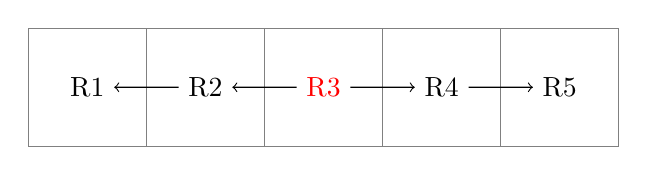
\begin{tikzpicture}[scale = 1.5]
\draw[color = gray] (0,0) grid[xstep = 1cm, ystep = 1cm] (5,1);
\node (R1) at (.5, .5) {R1};
\node (R2) at (1.5,.5) {R2};
\node (R3) [color =  red]  at (2.5,.5) {R3};
\node (R4) at (3.5,.5) {R4};
\node (R5) at (4.5,.5) {R5};
\draw [->] (R3) -- (R2);
\draw [->] (R3) -- (R4);
\draw [->] (R2) -- (R1);
\draw [->] (R4) -- (R5);
\end{tikzpicture}
\end{figure}
\end{frame}

\begin{frame}{Distance Matters}
\begin{alertblock}{Key Point:}
First law of geography of Waldo Tobler: \emph{``everything is related to everything else'', but near things are more related than distant things}
\end{alertblock}

This first law is the foundation of the fundamental concepts of \textbf{spatial dependence} and \textbf{spatial autocorrelation}.

\begin{figure}
	\caption{Professor Waldo Tobler}
\centering
	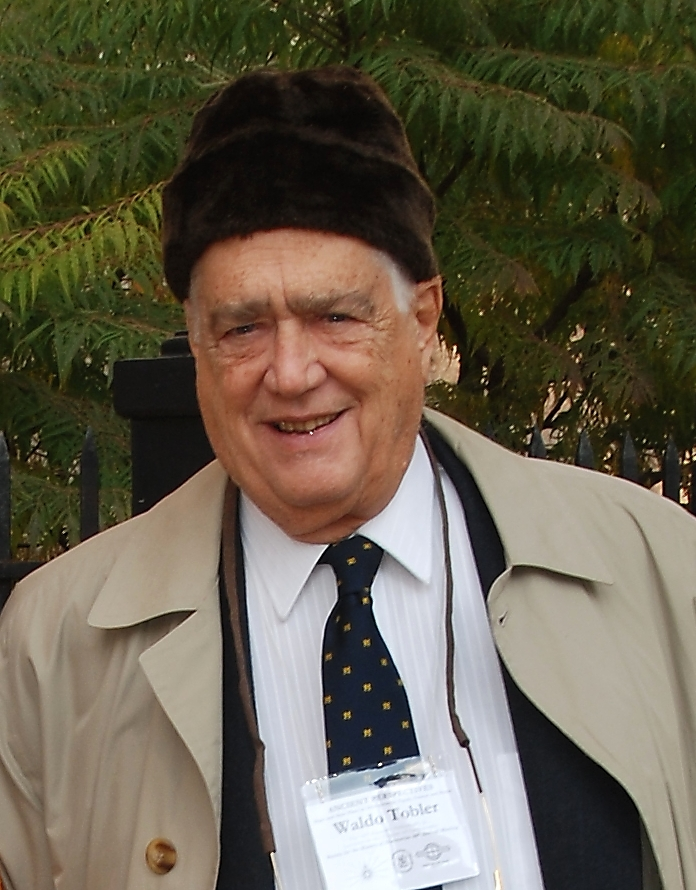
\includegraphics[width=4cm, height=4cm]{Waldo_Tobler}
\end{figure}

\end{frame}

%=====================================================
\subsection{Spatial Heterogeneity and Dependence}
%=====================================================



\begin{frame}
  \frametitle{Why do We Need Spatial Econometric?}
    \begin{itemize}
      \item Spatial econometric deals with \alert{spatial effects}
        \begin{enumerate}[(I)]
          \item<1-1> Spatial heterogeneity
          \item<2-2> Spatial dependence
        \end{enumerate}
    \end{itemize}
    
    \begin{definition}<1-1>[Spatial heterogeneity]
        Spatial heterogeneity relates to a \alert{differentiation} of the effects of space over the sample units. Formally, for spatial unit $i$:
        
        \begin{equation*}
          y_i = f(x_i)_i + \epsilon_i \implies y_i = \beta_i x_i + \epsilon_i
        \end{equation*}
        
    Lack of stability over the geographical space.
    \end{definition}

    \begin{definition}<2-2>[Spatial dependence]
       What happens in $i$ depends on what happens in $j$. Formally,
        \begin{equation*}
          y_i = f(y_i, y_j) + \epsilon_i, \forall i \neq j.
        \end{equation*}
    \end{definition}
\end{frame}


\begin{frame}
  \frametitle{Spatial Dependence}
    \begin{alertblock}{}
  How would you model this situation?
  \end{alertblock}
  
  \begin{figure}[h]
\caption{Environmental Externalities}
\label{fig:example_poll}
\centering
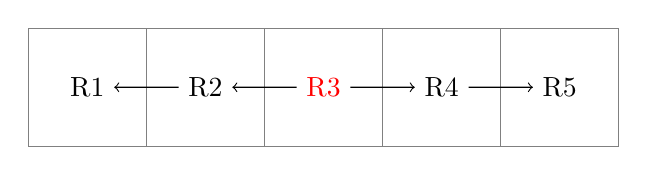
\begin{tikzpicture}[scale = 1.5]
\draw[color = gray] (0,0) grid[xstep = 1cm, ystep = 1cm] (5,1);
\node (R1) at (.5, .5) {R1};
\node (R2) at (1.5,.5) {R2};
\node (R3) [color =  red]  at (2.5,.5) {R3};
\node (R4) at (3.5,.5) {R4};
\node (R5) at (4.5,.5) {R5};
\draw [->] (R3) -- (R2);
\draw [->] (R3) -- (R4);
\draw [->] (R2) -- (R1);
\draw [->] (R4) -- (R5);
\end{tikzpicture}
\end{figure}
\end{frame}

\begin{frame}
  \frametitle{Spatial Dependence}
    Using our previous example, we would like to estimate 

\begin{equation}
  \begin{aligned}
y_1 & = \beta_{21} y_2 + \beta_{31} y_3 + \beta_{41} y_4 + \beta_{51} y_5 + \epsilon_1 \\
y_2 & = \beta_{12} y_1 + \beta_{32} y_3 + \beta_{42} y_4 + \beta_{52} y_5 + \epsilon_2 \\
y_3 & = \beta_{13} y_1 + \beta_{23} y_2 + \beta_{43} y_4 + \beta_{53} y_5 + \epsilon_3 \\
y_4 & = \beta_{14} y_1 + \beta_{24} y_2 + \beta_{34} y_3 + \beta_{54} y_5 + \epsilon_4 \\
y_5 & = \beta_{15} y_1 + \beta_{25} y_2 + \beta_{35} y_3 + \beta_{45} y_5 + \epsilon_4 
\end{aligned}
\end{equation}
%
where $\beta_{ji}$ is the effect of pollution of region $j$ on region $i$.
    
    \pause 
    \begin{alertblock}{}
    What is the problem with this modeling strategy?
    \end{alertblock}
\end{frame}


\begin{frame}
  \frametitle{Spatial Dependence}
  \begin{alertblock}{}
    Under standard econometric modeling, it is impossible to model spatial dependency.
  \end{alertblock}
\end{frame}

\subsection{Spatial Autocorrelation}


\begin{frame}
  \frametitle{Spatial Autocorrelation}
    \begin{itemize}
      \item <1-> Autocorrelation $\implies$ the correlation of a variables with itself
        \begin{itemize}
          \item<2-> Time series: the values of a variable at time $t$ depends on the value of the same variable at time $t-1$.
          \item<3-> Space: the correlation between the value of the variable at two different locations.
        \end{itemize}
    \end{itemize}



  \begin{definition}<4->[Spatial Autocorrelation]
    \begin{itemize}
      \item Correlation between the same attribute at two (or more) different locations.
      \item Coincidence of values similarity with location similarity.
      \item Under spatial dependency it is not possible to change the location of the values of certain variable without affecting the information in the sample. 
      \item It can be positive and negative.
    \end{itemize}
  \end{definition}
\end{frame}

\begin{frame}
  \frametitle{Spatial Autocorrelation}
    \begin{definition}[Positive Autocorrelation]
    Observations with high (or low) values of a variable tend to be clustered in space.
    \end{definition}

\pause    
\begin{figure}[h]
\caption{Positive Autocorrelation}
\centering
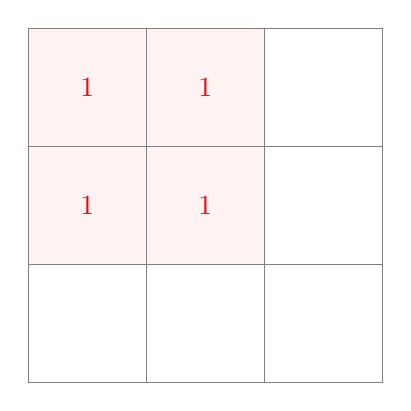
\begin{tikzpicture}[scale = 1.5]
\path [fill=red!5] (0,2) -- (1,2) -- (1,3) -- (0,3);
\path [fill=red!5] (1,2) -- (2,2) -- (2,3) -- (1,3);
\path [fill=red!5] (0,1) -- (1,1) -- (1,2) -- (0,2);
\path [fill=red!5] (1,1) -- (1,2) -- (2,2) -- (2,1);
\draw[color = gray] (0,0) grid[xstep = 1cm, ystep = 1cm] (3,3); % grid of 3 times 3
\node [color =  red] at (.5, 2.5) {1};
\node [color =  red] at (1.5, 2.5) {1};
\node at (2.5, 2.5) {};
\node [color =  red] at (.5, 1.5) {1};
\node [color =  red] at (1.5,1.5) {1} ;
\node at (2.5,1.5) {};
\node at (.5, .5) {};
\node at (1.5,.5) {};
\node at (2.5,.5) {};
\end{tikzpicture}
\end{figure}
\end{frame}

\begin{frame}
  \frametitle{Spatial Autocorrelation}
    \begin{definition}[Negative Autocorrelation]
    Locations tend to be surrounded by neighbors having very dissimilar values.
    \end{definition}

\pause    
\begin{figure}[h]
\caption{Negative Autocorrelation}
\centering
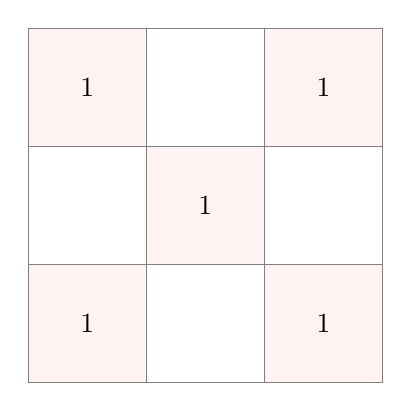
\begin{tikzpicture}[scale = 1.5]
\path [fill=red!5] (0,2) -- (1,2) -- (1,3) -- (0,3);
\path [fill=red!5] (0,0) -- (1,0) -- (1,1) -- (0,1);
\path [fill=red!5] (2,2) -- (3,2) -- (3,3) -- (2,3);
\path [fill=red!5] (2,0) -- (3,0) -- (3,1) -- (2,1);
\path [fill=red!5] (1,1) -- (1,2) -- (2,2) -- (2,1);
\draw[color = gray] (0,0) grid[xstep = 1cm, ystep = 1cm] (3,3); % grid of 3 times 3
\node at (.5, 2.5) {1};
\node at (1.5, 2.5) {};
\node at (2.5, 2.5) {1};
\node at (.5, 1.5) {};
\node at (1.5,1.5) {1} ;
\node at (2.5,1.5) {};
\node at (.5, .5) {1};
\node at (1.5,.5) {};
\node at (2.5,.5) {1};
\end{tikzpicture}
\end{figure}
\end{frame}


\begin{frame}[fragile]
  \frametitle{Spatial Autocorrelation: Another Example}
\begin{knitrout}
\definecolor{shadecolor}{rgb}{0.969, 0.969, 0.969}\color{fgcolor}

{\centering 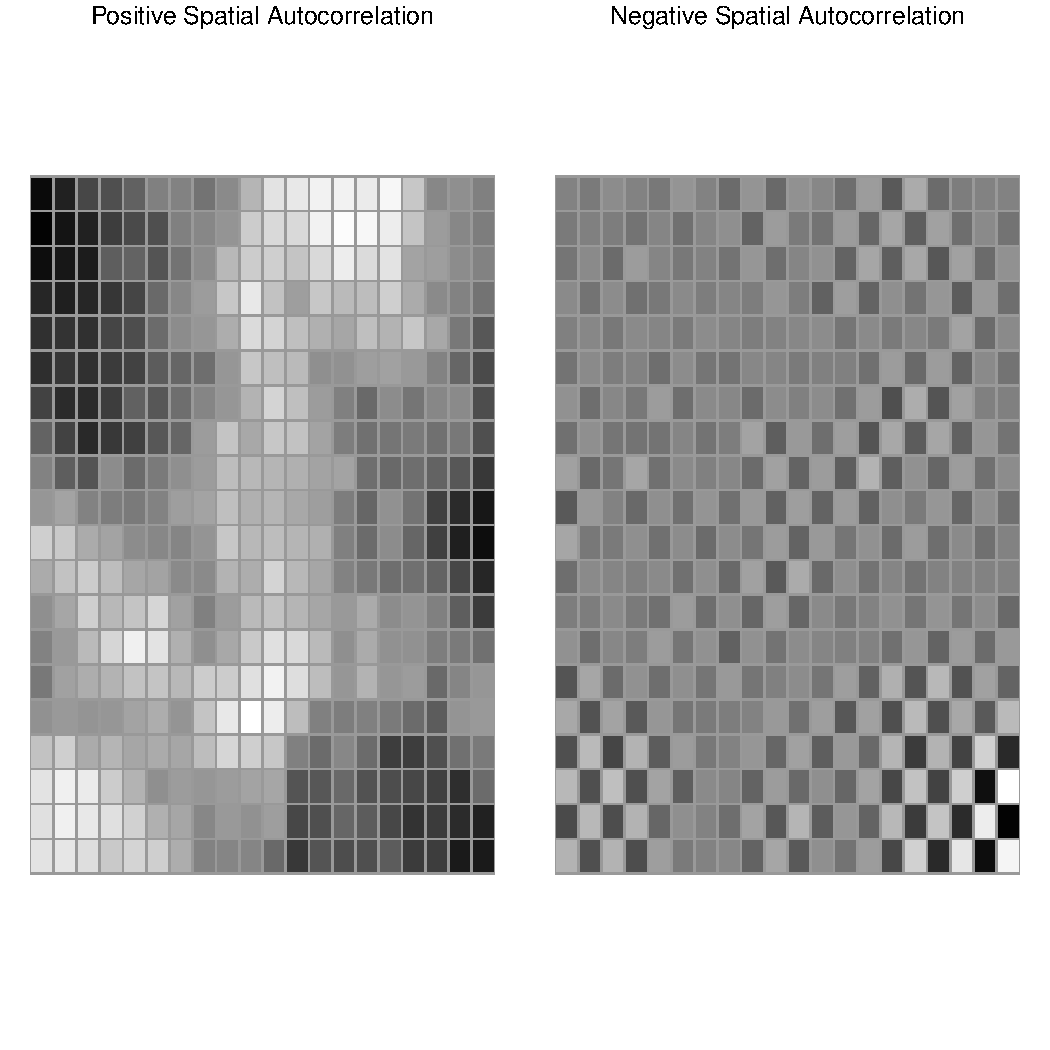
\includegraphics[width=8cm,height=8cm]{figure/plot_spatial_auto-1} 

}


\end{knitrout}
\end{frame}


\begin{frame}
  \frametitle{Spatial Autocorrelation}
    \begin{definition}[Spatial Randomness]
    When none of the two situations occurs.
    \end{definition}
\end{frame}

\begin{frame}
  \frametitle{Spatial Autocorrelation}
    Two main sources of spatial autocorrelation (Anselin, 1988):
      \begin{itemize}
        \item Measurement errors.
        \item Importance of Space.
      \end{itemize}
      
    The second source is of much more interest.
    
    \begin{figure}
	\caption{Professor Luc Anselin}
\centering
	
\includegraphics[width=5cm, height=5cm]{luc_anselin}
\end{figure}
\end{frame}

\begin{frame}
  \frametitle{Why the space matters?}
    \begin{itemize}
      \item The essence of regional sciences and new economic geography is that \alert{location and distance matter}.
      \item What is observed at one point is determined by what happen elsewhere in the system.
    \end{itemize}
\end{frame}


\begin{frame}
  \frametitle{First Law of Geography Again}
    \begin{alertblock}<1->{Tobler's First Law of Geography}
      \emph{Everything depends on everything else, but closer things more so}
    \end{alertblock}
    
    \begin{itemize}[<+->]
      \item Important ideas:
        \begin{itemize}
          \item \alert{Existence} of Spatial Dependence.
          \item \alert{Structure} of Spatial Dependence
            \begin{itemize}
              \item Distance decay.
              \item Closeness =  Similarities.
            \end{itemize}
        \end{itemize}
    \end{itemize}
\end{frame}


%********************************
\section{Spatial Weight Matrix}
%********************************

\subsection{Definition}

\begin{frame}
  \frametitle{Spatial Weight Matrix}
One crucial issue in spatial econometric is the problem of formally incorporating spatial dependence into the model.
  
  \pause  
  \begin{alertblock}{Question?}
  What would be a good criteria to define closeness in space? Or, in other words, how to determine which other units in the system influence the one under consideration?
  \end{alertblock}

\end{frame}

\begin{frame}
  \frametitle{Spatial Weight Matrix}
    \begin{itemize}
      \item The device typically used in spatial analysis is the so-called \alert{spatial weight matrix}, or simply $\mW$ matrix.
      \item Impose a \alert{structure} in terms of what are the \alert{neighbors} for each location.
      \item Assigns \alert{weights} that measure the \alert{intensity of the relationship} among pair of spatial units.
      \item Not necessarily \alert{symmetric}.
    \end{itemize}
\end{frame}

\begin{frame}
  \frametitle{Spatial Weight Matrix}
    \begin{definition}[$\mW$ Matrix]
      Let $n$ be the number of spatial units. The spatial weight matrix, $\mW$, a $n\times n$ positive symmetric and \textbf{non-stochastic} matrix with element $w_{ij}$ at location $i,j$. The values of $w_{ij}$ or the weights for each pair of locations are assigned by some preset rules which defines the spatial relations among locations. By convention, $w_{ij} = 0$ for the diagonal elements.
    \end{definition}
    \alert{The symmetry assumption can be dropped later.} 
    \begin{equation*}
\mW = \begin{pmatrix}
        w_{11} & w_{12} & \hdots & w_{1n} \\ 
        w_{21} & w_{22} & \hdots & w_{2n} \\
        \vdots & \vdots & \ddots & \vdots \\
        w_{n1} & w_{n2} & \hdots & w_{nn} 
      \end{pmatrix}
\end{equation*}
\end{frame}


\begin{frame}
  \frametitle{Spatial Weight Matrix}
  Two main approaches:
    \begin{enumerate}
      \item Contiguity.
      \item Based on distance
    \end{enumerate}
\end{frame}

%==========================================
\subsection{Weights Based on Boundaries}
%==========================================



\begin{frame}
  \frametitle{Weights Based on Boundaries}
  The availability of polygon or lattice data permits the construction of contiguity-based spatial weight matrices. A typical specification of the contiguity relationship in the spatial weight matrix is

\begin{equation}
  w_{ij}= 
   \begin{cases}
      1 & \mbox{if $i$ and $j$ are contiguous} \\ 
      0 & \mbox{if $i$ and $j$ are not contiguous} 
   \end{cases}
\end{equation}

  \begin{enumerate}
    \item Binary Contiguity:
      \begin{itemize}
        \item Rook criterion (Common Border)
        \item Bishop criterion (Common Vertex)
        \item Queen criterion (Either common border or vertex)
      \end{itemize}
  \end{enumerate}
\end{frame}


\begin{frame}
  \frametitle{Rook Contiguity}
  
  How are the neighbors of region 5?
  
\begin{figure}[h]
\caption{Rook Contiguity}
\label{fig:Rook_cont_grid}
\centering
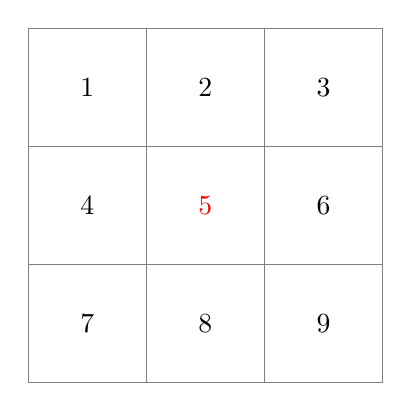
\begin{tikzpicture}[scale = 1.5]
\path  (1,2) -- (2,2) -- (2,3) -- (1,3);
\path  (1,0) -- (2,0) -- (2,1) -- (1,1);
\path  (0,1) -- (1,1) -- (1,2) -- (0,2);
\path  (2,1) -- (3,1) -- (3,2) -- (2,2);
\draw[color = gray] (0,0) grid[xstep = 1cm, ystep = 1cm] (3,3); % grid of 3 times 3
\node at (.5, 2.5) {1};
\node at (1.5, 2.5) {2};
\node at (2.5, 2.5) {3};
\node at (.5, 1.5) {4};
\node [color =  red] at (1.5,1.5) {5} ;
\node at (2.5,1.5) {6};
\node at (.5, .5) {7};
\node at (1.5,.5) {8};
\node at (2.5,.5) {9};
\end{tikzpicture}
\end{figure}
\end{frame}
		
\begin{frame}
  \frametitle{Rook Contiguity}
\begin{figure}[h]
\caption{Rook Contiguity}
\label{fig:Rook_cont_grid}
\centering
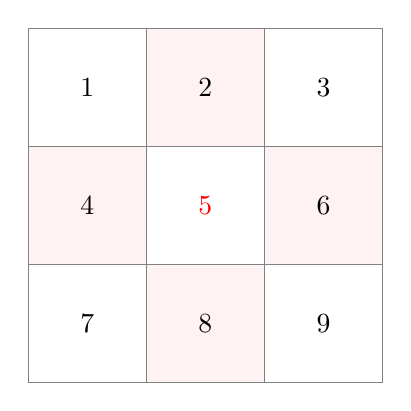
\begin{tikzpicture}[scale = 1.5]
\path [fill=red!5] (1,2) -- (2,2) -- (2,3) -- (1,3);
\path [fill=red!5] (1,0) -- (2,0) -- (2,1) -- (1,1);
\path [fill=red!5] (0,1) -- (1,1) -- (1,2) -- (0,2);
\path [fill=red!5] (2,1) -- (3,1) -- (3,2) -- (2,2);
\draw[color = gray] (0,0) grid[xstep = 1cm, ystep = 1cm] (3,3); % grid of 3 times 3
\node at (.5, 2.5) {1};
\node at (1.5, 2.5) {2};
\node at (2.5, 2.5) {3};
\node at (.5, 1.5) {4};
\node [color =  red] at (1.5,1.5) {5} ;
\node at (2.5,1.5) {6};
\node at (.5, .5) {7};
\node at (1.5,.5) {8};
\node at (2.5,.5) {9};
\end{tikzpicture}
\end{figure}

\pause Common border: 2, 4, 5, 6
\end{frame}
		
\begin{frame}
  \frametitle{Bishop Contiguity}
\begin{figure}[h]
\caption{Bishop Contiguity}
\label{fig:Bishop_cont_grid}
\centering
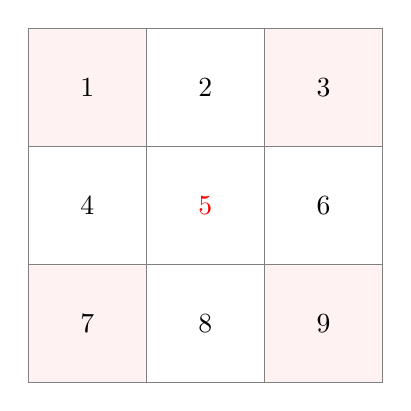
\begin{tikzpicture}[scale = 1.5]
\path [fill=red!5] (0,2) -- (1,2) -- (1,3) -- (0,3);
\path [fill=red!5] (0,0) -- (1,0) -- (1,1) -- (0,1);
\path [fill=red!5] (2,2) -- (3,2) -- (3,3) -- (2,3);
\path [fill=red!5] (2,0) -- (3,0) -- (3,1) -- (2,1);
\draw[color = gray] (0,0) grid[xstep = 1cm, ystep = 1cm] (3,3); % grid of 3 times 3
\node at (.5, 2.5) {1};
\node at (1.5, 2.5) {2};
\node at (2.5, 2.5) {3};
\node at (.5, 1.5) {4};
\node [color =  red] at (1.5,1.5) {5} ;
\node at (2.5,1.5) {6};
\node at (.5, .5) {7};
\node at (1.5,.5) {8};
\node at (2.5,.5) {9};
\end{tikzpicture}
\end{figure}


\pause Common vertex: 1, 3, 7, 9
\end{frame}


\begin{frame}
  \frametitle{Queen Contiguity}
\begin{figure}[h]
\caption{Queen Contiguity}
\label{fig:Queen_cont_grid}
\centering
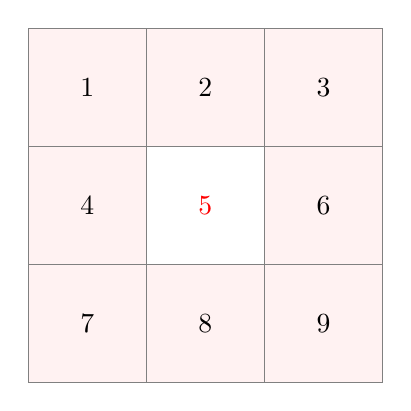
\begin{tikzpicture}[scale = 1.5]
\path [fill=red!5] (0,2) -- (1,2) -- (1,3) -- (0,3);
\path [fill=red!5] (0,0) -- (1,0) -- (1,1) -- (0,1);
\path [fill=red!5] (2,2) -- (3,2) -- (3,3) -- (2,3);
\path [fill=red!5] (2,0) -- (3,0) -- (3,1) -- (2,1);
\path [fill=red!5] (1,2) -- (2,2) -- (2,3) -- (1,3);
\path [fill=red!5] (1,0) -- (2,0) -- (2,1) -- (1,1);
\path [fill=red!5] (0,1) -- (1,1) -- (1,2) -- (0,2);
\path [fill=red!5] (2,1) -- (3,1) -- (3,2) -- (2,2);
\draw[color = gray] (0,0) grid[xstep = 1cm, ystep = 1cm] (3,3); % grid of 3 times 3
\node at (.5, 2.5) {1};
\node at (1.5, 2.5) {2};
\node at (2.5, 2.5) {3};
\node at (.5, 1.5) {4};
\node [color =  red] at (1.5,1.5) {5} ;
\node at (2.5,1.5) {6};
\node at (.5, .5) {7};
\node at (1.5,.5) {8};
\node at (2.5,.5) {9};
\end{tikzpicture}
\end{figure}


\pause Common vertex and border: 1, 2, 3, 4, 6, 7, 8, 9.
\end{frame}

%================================================
\subsection{From Contiguity to the W Matrix}
%=================================================


\begin{frame}
  \frametitle{Rook Contiguity}
  \begin{columns}
    \begin{column}{.1\textwidth}
\begin{flushleft}
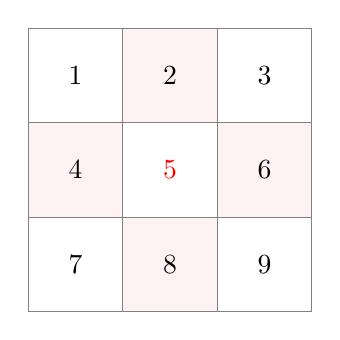
\begin{tikzpicture}[scale = 1.2]
\path [fill=red!5] (1,2) -- (2,2) -- (2,3) -- (1,3);
\path [fill=red!5] (1,0) -- (2,0) -- (2,1) -- (1,1);
\path [fill=red!5] (0,1) -- (1,1) -- (1,2) -- (0,2);
\path [fill=red!5] (2,1) -- (3,1) -- (3,2) -- (2,2);
\draw[color = gray] (0,0) grid[xstep = 1cm, ystep = 1cm] (3,3); % grid of 3 times 3
\node at (.5, 2.5) {1};
\node at (1.5, 2.5) {2};
\node at (2.5, 2.5) {3};
\node at (.5, 1.5) {4};
\node [color =  red] at (1.5,1.5) {5} ;
\node at (2.5,1.5) {6};
\node at (.5, .5) {7};
\node at (1.5,.5) {8};
\node at (2.5,.5) {9};
\end{tikzpicture}
\end{flushleft}
    \end{column}

    \begin{column}{.3\textwidth}
        \begin{equation*}
  \mW = 
  \begin{pmatrix}
     0 & 1 & 0 & 1 & 0 & 0 & 0 & 0 & 0 \\
     1 & 0 & 1 & 0 & 1 & 0 & 0 & 0 & 0 \\
     0 & 1 & 0 & 0 & 0 & 1 & 0 & 0 & 0 \\
     1 & 0 & 0 & 0 & 1 & 0 & 1 & 0 & 0 \\
     \alert{0} & \alert{1} & \alert{0} & \alert{1} & \alert{0} & \alert{1} & \alert{0} & \alert{1} & \alert{0} \\
     0 & 0 & 1 & 0 & 1 & 0 & 0 & 0 & 1 \\
     0 & 0 & 0 & 1 & 0 & 0 & 0 & 1 & 0 \\
     0 & 0 & 0 & 0 & 1 & 0 & 1 & 0 & 1 \\
     0 & 0 & 0 & 0 & 0 & 1 & 0 & 1 & 0 \\
  \end{pmatrix}
\end{equation*}
    \end{column}
\end{columns}
\end{frame}

\begin{frame}
  \frametitle{Bishop Contiguity}

  \begin{columns}
    \begin{column}{.1\textwidth}
\begin{flushleft}
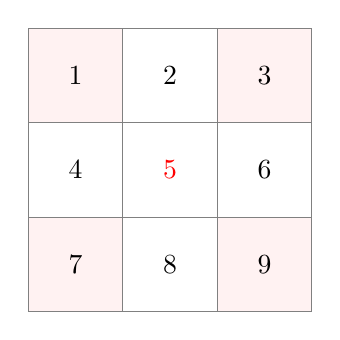
\begin{tikzpicture}[scale = 1.2]
\path [fill=red!5] (0,2) -- (1,2) -- (1,3) -- (0,3);
\path [fill=red!5] (0,0) -- (1,0) -- (1,1) -- (0,1);
\path [fill=red!5] (2,2) -- (3,2) -- (3,3) -- (2,3);
\path [fill=red!5] (2,0) -- (3,0) -- (3,1) -- (2,1);
\draw[color = gray] (0,0) grid[xstep = 1cm, ystep = 1cm] (3,3); % grid of 3 times 3
\node at (.5, 2.5) {1};
\node at (1.5, 2.5) {2};
\node at (2.5, 2.5) {3};
\node at (.5, 1.5) {4};
\node [color =  red] at (1.5,1.5) {5} ;
\node at (2.5,1.5) {6};
\node at (.5, .5) {7};
\node at (1.5,.5) {8};
\node at (2.5,.5) {9};
\end{tikzpicture}
\end{flushleft}
    \end{column}

    \begin{column}{.3\textwidth}
\begin{equation*}
\mW = 
  \begin{pmatrix}
     0 & 0 & 0 & 0 & 1 & 0 & 0 & 0 & 0 \\
     0 & 0 & 0 & 1 & 0 & 1 & 0 & 0 & 0 \\
     0 & 0 & 0 & 0 & 1 & 0 & 0 & 0 & 0 \\
     0 & 1 & 0 & 0 & 0 & 0 & 0 & 1 & 0 \\
     \alert{1} & \alert{0} & \alert{1} & \alert{0} & \alert{0} & \alert{0} & \alert{1} & \alert{0} & \alert{1} \\
     0 & 1 & 0 & 0 & 0 & 0 & 0 & 1 & 0 \\
     0 & 0 & 0 & 0 & 1 & 0 & 0 & 0 & 0 \\
     0 & 0 & 0 & 1 & 0 & 1 & 0 & 0 & 0 \\
     0 & 0 & 0 & 0 & 1 & 0 & 0 & 0 & 0 \\
  \end{pmatrix}
\end{equation*}
    \end{column}
\end{columns}
\end{frame}

%==========================================
\subsection{Weights Based on Distance}
%==========================================

\begin{frame}
  \frametitle{$\mW$ based on distance}
    \begin{itemize}
      \item Weights may be also defined as a function of the distance between region $i$ and $j$, $d_{ij}$.
      \item $d_{ij}$ is usually computed as the distance between their centroids (or other important unit).
      \item Let $x_i$ an $x_j$ be the longitud and $y_i$ and $y_j$ the latitude coordinates for region $i$ and $j$, respectively:
    \end{itemize}
\end{frame}

\begin{frame}
  \frametitle{Distance Metric}
  \begin{definition}[Minkowski metric]
    Let two point $i$ and $j$, with respective coordinates $(x_i, y_i)$ and $(x_j, y_j)$:
    \begin{equation}
  d_{ij}^p = \left(\left|x_i - x_j\right|^p + \left|y_i - y_j\right|^p\right)^{1/p}
\end{equation}
  \end{definition}
  
    \begin{definition}[Euclidean metric]
    Consider Minkowski metric and set $p = 2$, then
    
    \begin{equation}
  d_{ij}^e = \sqrt{(x_i - x_j)^2 + (y_i - y_j)^2}.
\end{equation}
  \end{definition}
  
\begin{definition}[Manhattan metric]
  Consider Minkowski metric and set $p = 1$, then
  
  \begin{equation}
   d_{ij}^m = \left|x_i - x_j\right| + \left|y_i - y_j\right|.
\end{equation}
\end{definition}
\end{frame}

\begin{frame}
  \frametitle{Distance Metric}
    \begin{itemize}
      \item Euclidean distance is not necessarily the shortest distance if you take into account the curvature of the earth. 
    \end{itemize}
    
    \begin{definition}[Great Circle Distance]
    Let two point $i$ and $j$, with respective coordinates $(x_i, y_i)$ and $(x_j, y_j)$:
    \begin{equation}
d_{ij}^{cd} = r \times \arccos^{-1}\left[\cos|x_i - x_j| \cos y_i \cos y_j + \sin y_i \sin y_j \right]
\end{equation}
%
where $r$ is the Earth's radius. The arc distance is obtained in miles with $r = 3959$ and in kilometers with $r = 6371$.
    \end{definition}
\end{frame}


\begin{frame}
  \frametitle{$\mW$ based on distance}
    \begin{itemize}
      \item Inverse distance:
      \begin{equation}
  w_{ij} =
  \begin{cases}
  \frac{1}{d_{ij}^{\alpha}} & \mbox{if} \;\;i \neq j \\
  0 & \mbox{if}\;\; i = j
  \end{cases}
\end{equation}
Typically, $\alpha = 1$ or $\alpha = 2$.
\item Negative exponential model:
\begin{equation}
  w_{ij} = \exp\left(-\frac{d_{ij}}{\alpha}\right)
\end{equation}
    \end{itemize}
\end{frame}

\begin{frame}
  \frametitle{$\mW$ based on distance}
\begin{knitrout}
\definecolor{shadecolor}{rgb}{0.969, 0.969, 0.969}\color{fgcolor}

{\centering 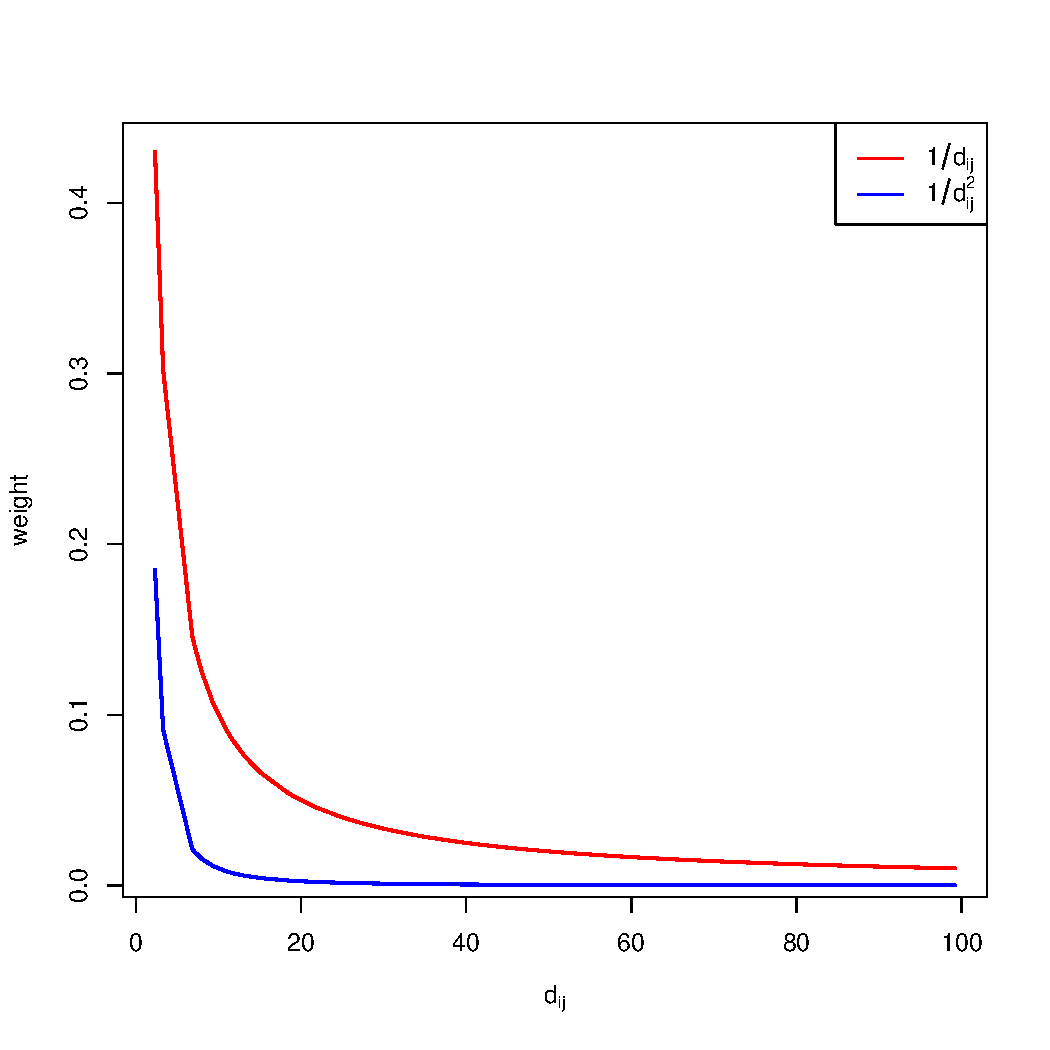
\includegraphics[width=8cm,height=8cm]{figure/dist-graph-1} 

}


\end{knitrout}
  
\end{frame}

\begin{frame}
  \frametitle{$\mW$ based on distance}
    \begin{itemize}
      \item $k$-nearest neighbors: We explicitly limit the number of neighbors. 
      \begin{equation}
  w_{ij} =
  \begin{cases}
  1 & \mbox{if centroid of $j$ is one of the $k$ nearest centroids to that of $i$}  \\
  0 & \mbox{otherwise}
  \end{cases}
\end{equation}

\item Threshold Distance (Distance Band Weights): In contrast to the $k$-nearest neighbors method, the threshold distance specifies that an region $i$ is neighbor of $j$ if the distance between them is less than a specified maximum distance:


\begin{equation}
  w_{ij}= 
   \begin{cases}
      1 & \mbox{if}\;\; 0\leq d_{ij} \leq d_{max} \\ 
      0 & \mbox{if}\;\; d_{ij} > d_{max}
   \end{cases}
\end{equation}


To avoid isolates that would result from too stringent a critical distance, the distance must be chosen such that each location has at least one neighbor. Such a distance conforms to a max-min criterion, i.e., it is the largest of the nearest neighbor distances.
\end{itemize}
\end{frame}

%================================
\subsection{Row Standardization}
%================================

\begin{frame}
  \frametitle{Row standardization}
    \begin{itemize}
      \item $\mW$'s are used to compute \alert{weighted averages} in which more weight is placed on nearby observations than on distant observations.
      \item The elements of a row-standardized weights matrix equal

\begin{equation*}
w_{ij}^s = \frac{w_{ij}}{\sum_j w_{ij}}.
\end{equation*}

This ensures that all weights are between 0 and 1 and facilities the interpretation of operation with the weights matrix as an averaging of neighboring values. 
\item Under row-standardization, the element of each \alert{row sum} to unity.  
\item The row-standardized weights matrix also ensures that the \alert{spatial parameter} in many spatial stochastic processes are comparable between models.
\item Under row-standardization the matrices are not longer \alert{symmetric}!.
\end{itemize}
\end{frame}

\begin{frame}
  \frametitle{Row standardization}
  The row-standardized matrix is also known in the literature as the row-stochastic matrix:
  
  \begin{definition}[Row-stochastic Matrix]
	A real $n\times n$ matrix $\mA$ is called \textbf{Markov} matrix, or \textbf{row-stochastic matrix} if 
		\begin{enumerate}
			\item $a_{ij} \geq 0$ for $1\leq i, j \leq n$;
			\item $\sum_{j=1}^n a_{ij} = 1$ for $1\leq i \leq n$
		\end{enumerate}
\end{definition}

An important characteristic of the row-stochastic matrix is related to its eigen values:

\begin{theorem}[Eigenvalues of row-stochastic Matrix]\label{teo:eigen_values}
	Every eigenvalue $\omega_i$ of a row-stochastic Matrix satisfies $\left|\vomega\right|\leq 1$
\end{theorem}

Therefore, the eigenvalues of the row-stochastic (i.e., row-normalized, row standardized or Markov) neighborhood matrix $\mW^s$ are in the range $\left[-1, +1\right]$.
\end{frame}


%==========================================
\subsection{Spatial Lag}
%==========================================

\begin{frame}
  \frametitle{Spatial Lag}
The spatial lag operator takes the form $\vy_L = \mW\vy$ with dimension $n \times 1$, where each element is given by $\vy_{Li} = \sum_{j}w_{ij}y_j$, i.e., a weighted average of the $\vy$ values in the neighbor of $i$.

For example:


\begin{equation}
  \mW\vy =    \begin{pmatrix}
     0 & 1 & 0 \\
     1 & 0 & 1 \\
     0 & 1 & 0
  \end{pmatrix}
  \begin{pmatrix}
     10 \\
     50 \\
     30
  \end{pmatrix} =
  \begin{pmatrix}
     50 \\
     10 + 30 \\
     50
  \end{pmatrix}
\end{equation}

Using a row-standardized weight matrix:

\begin{equation}
  \mW^s\vy =    \begin{pmatrix}
     0 & 1 & 0 \\
     0.5 & 0 & 0.5 \\
     0 & 1 & 0
  \end{pmatrix}
  \begin{pmatrix}
     10 \\
     50 \\
     30
  \end{pmatrix} =
  \begin{pmatrix}
     50 \\
     5 + 15 \\
     50
  \end{pmatrix}
\end{equation}

Therefore, when $\mW$ is standardized, each element $(\mW^s\vy)_i$ is interpreted as a weighted average of the $y$ values for $i$'s neighbors. 

\end{frame}


%==========================================
\subsection{Higher-Order Spatial Neighbors}
%==========================================

\begin{frame}{Higher-Order Neighbors}
  \begin{itemize}
    \item How to define higher-order neighbors?
      \begin{itemize}
        \item We might be interested in the neighbors of the neighbors of spatial unit $i$.
      \end{itemize}
    \item We define the higher-order spatial weigh matrix $l$ as $\mW^l$.
    \begin{itemize}
          \item Spatial weight of order $l = 2$ is given by $\mW^2= \mW\mW$.
          \item Spatial weight of order $l = 3$ is given by $\mW^3= \mW\mW\mW$.
        \end{itemize}
    \item As an illustration consider the following structure for our previous example:


\begin{equation}\label{eq:W5x5}
\mW = \begin{pmatrix}
      0 & 1 & 0 & 0 & 0 \\
      1 & 0 & 1 & 0 & 0 \\
      0 & 1 & 0 & 1 & 0 \\
      0 & 0 & 1 & 0 & 1 \\
      0 & 0 & 0 & 1 & 0
      \end{pmatrix}
\end{equation}
  \end{itemize}
\end{frame}

\begin{frame}{Higher-Order Neighbors}
Then $\mW^2 = \mW\mW$ based on the $5\times 5$ first-order contiguity matrix $\mW$ from (\ref{eq:W5x5}) is:

\begin{equation}
\mW^2 = \begin{pmatrix}\label{eq:W25x5}
      1 & 0 & 1 & 0 & 0 \\
      0 & 2 & 0 & 1 & 0 \\
      1 & 0 & 2 & 0 & 1 \\
      0 & 1 & 0 & 2 & 0 \\
      0 & 0 & 1 & 0 & 1
      \end{pmatrix}
\end{equation}

\begin{figure}[ht]
\caption{Higher-Order Neighbors}
\label{fig:example_hon}
\centering
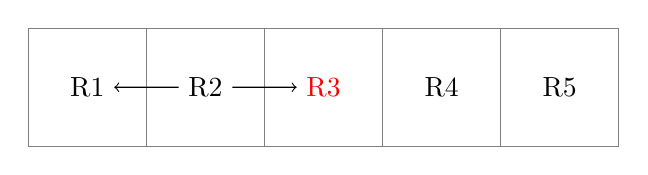
\begin{tikzpicture}[scale = 1.5]
\draw[color = gray] (0,0) grid[xstep = 1cm, ystep = 1cm] (5,1);
\node (R1) at (.5, .5) {R1};
\node (R2) at (1.5,.5) {R2};
\node (R3) [color =  red]  at (2.5,.5) {R3};
\node (R4) at (3.5,.5) {R4};
\node (R5) at (4.5,.5) {R5};
\draw [->] (R2) -- (R1);
\draw [->] (R2) -- (R3);
\end{tikzpicture}
\\
\vspace{1cm}
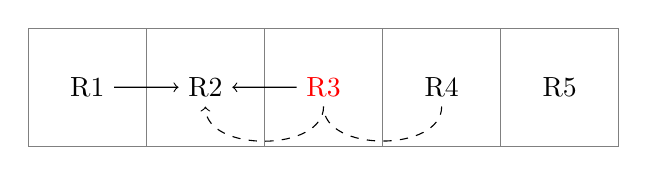
\begin{tikzpicture}[scale = 1.5]
\draw[color = gray] (0,0) grid[xstep = 1cm, ystep = 1cm] (5,1);
\node (R1) at (.5, .5) {R1};
\node (R2) at (1.5,.5) {R2};
\node (R3) [color =  red]  at (2.5,.5) {R3};
\node (R4) at (3.5,.5) {R4};
\node (R5) at (4.5,.5) {R5};
\draw [->] (R1) -- (R2);
\draw [->] (R3) -- (R2);
\draw [->, dashed] (R4) to[out= 270,in=270] (R3) to[out=270,in=270] (R2);
\end{tikzpicture}
\end{figure}
\end{frame}



%***********************************************
\section{Testing for Spatial Autocorrelation}
%***********************************************

\subsection{Indicators of spatial association}

\begin{frame}
  \frametitle{Global Autocorrelation}
    \begin{itemize}
      \item Indicators of spatial association
        \begin{enumerate}
          \item Global Autocorrelation
          \item Local Autocorrelation
        \end{enumerate}
    \end{itemize}
    \begin{definition}[Global Autocorrelation]
      It is a measure of overall clustering in the data. It yields only one statistic to summarize the whole study area (Homogeneity).
        \begin{enumerate}
          \item Moran's I.
          \item Gery's $C$.
          \item Getis and Ord's $G(d)$
        \end{enumerate}
    \end{definition}
        \begin{definition}[Local Autocorrelation]
        A measure of spatial autocorrelation for each individual location.
          \begin{itemize}
            \item Local Indices for spatial Spatial Analysis (LISA)
          \end{itemize}
    \end{definition}
\end{frame}

%========================
\subsection{Moran's I}
%========================

\begin{frame}
  \frametitle{Moran's I}
    This statistic is given by:
      \begin{equation}
I = \frac{\sum_{i = 1}^n\sum_{j=1, j\neq i}^n w_{ij}\left(x_i - \bar{x}\right)\left(x_j - \bar{x}\right)}{S_0 \sum_{i = 1}^n\left(x_i - \bar{x}\right)^2/n} = \frac{n\sum_{i = 1}^n\sum_{j=1}^n w_{ij}\left(x_i - \bar{x}\right)\left(x_j - \bar{x}\right)}{S_0 \sum_{i = 1}^n\left(x_i - \bar{x}\right)^2}
\end{equation}

where $S_0=\sum_{i = 1}^n\sum_{j=1}^nw_{ij}$ and $w_{ij}$ is an element of the spatial weight matrix that measures spatial distance or connectivity between regions $i$ and $j$. In matrix form:


\begin{equation}
	I = \frac{n}{S_0} \frac{\vz^\top\mW\vz}{\vz^\top\vz}
\end{equation}

where $\vz = \vx - \bar{x}$. If the $\mW$ matrix is row standardized, then:

\begin{equation}
	I = \frac{\vz^\top\mW^s\vz}{\vz^\top\vz}
\end{equation}

because $S_0=n$. Values range from -1 (perfect dispersion) to +1 (perfect correlation). A zero value indicates a random spatial pattern.
\end{frame}

\begin{frame}
  \frametitle{Moran Scatterplot}
    \begin{itemize}
      \item A very useful tool for understanding the Moran's I test
    \end{itemize}
    

\begin{knitrout}
\definecolor{shadecolor}{rgb}{0.969, 0.969, 0.969}\color{fgcolor}

{\centering 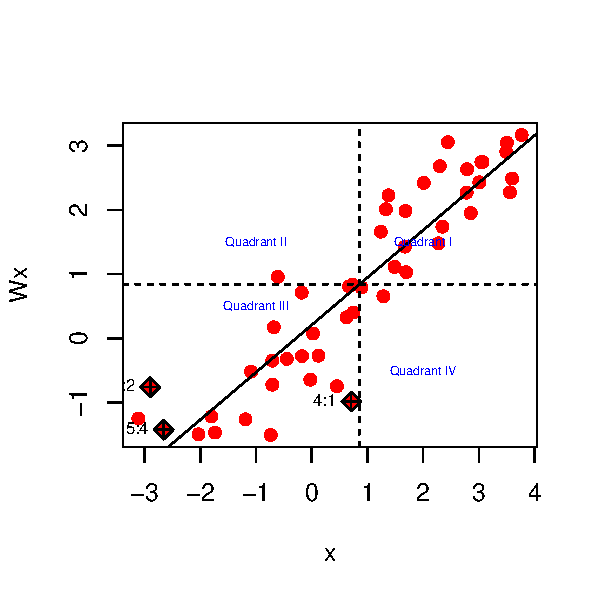
\includegraphics[width=0.7\linewidth]{figure/moran-1} 

}


\end{knitrout}

\end{frame}

\begin{frame}
  \frametitle{Moran's I}
    Note that:
        \begin{equation*}
          \widehat{\beta}_{OLS} = \frac{\sum_i(x_i -\bar{x})(y_i - \bar{y})}{\sum_i(x_i - \bar{x})^2}
        \end{equation*}
        
        \alert{Therefore?}
        
        \pause
        \begin{alertblock}{Remark}
        $I$ is equivalent to the slope coefficient of a linear regression of the spatial lag $\mW\vx$ on the observation vector $\vx$ measured in deviation from their means. It is, however, not equivalent to the slope of $\vx$ on $\mW\vx$ which would be a more natural way.
        \end{alertblock}
\end{frame}

\begin{frame}
  \frametitle{Moran's I}
    \begin{itemize}
      \item $H_0$: $x$ is spatially independent, the observed $x$ are assigned at random among locations. ($I$ is close to zero)
      \item $H_1$: $X$ is not spatially independent. ($I$ is not zero)
    \end{itemize}
\end{frame}

\begin{frame}
  \frametitle{Moran's I}
    \begin{itemize}
      \item We are interested in the distribution of the following statistic:
            \begin{equation}
              T_I = \frac{I - \E(I)}{\sqrt{\var(I)}}
            \end{equation}
      \item Three approaches to compute the variance of Moran's $I$:
        \begin{itemize}
          \item Monte Carlo
          \item Normality of $x_i$: It is assumed that the random variable $x_i$ are the result of $n$ independently drawings from a normal population.
          \item Randomization of $x_i$: No matter what the underlying distribution of the population, we consider the observed values of $x_i$ were repeatedly randomly permuted.
        \end{itemize}
    \end{itemize}
\end{frame}

\begin{frame}
  \frametitle{Moran's I}
    \begin{theorem}[Moran's $I$ Under Normality]\label{teo:Moran_normal}
Assume that $\left\lbrace \vx_i\right\rbrace = \left\lbrace x_1, x_2,..., x_n\right\rbrace$ are independent and distributed as $\rN(\mu, \sigma^2)$, but $\mu$ and $\sigma^2$ are unknown. Then:

\begin{equation}
\E\left(I\right) = - \frac{1}{n - 1} 
\end{equation}
%
and

\begin{equation}
\E\left(I^2\right) = \frac{n^2S_1 - nS_2 + 3S_0^2}{S_0^2(n^2 - 1)}
\end{equation}
%
where $S_0=\sum_{i = 1}^n\sum_{j=1}^nw_{ij}$, $S_1= \sum_{i = 1}^n\sum_{j = 1}^n(w_{ij} + w_{ji})^2/2$, $S_2 = \sum_{i = 1}^n(w_{i.} + w_{.i})^2$, where $w_{i.}= \sum_{j = 1}^nw_{ij}$ and $w_{i.}=\sum_{j = 1}^nw_{ji}$
Then:

\begin{equation}
\var\left(I\right)=\E\left(I^2\right) - \E\left(I\right)^2
\end{equation}
\end{theorem}
\end{frame}

\begin{frame}
  \frametitle{Moran's I}
  Theorem \ref{teo:Moran_random} gives the moments of Moran's I under randomization. 


\begin{theorem}[Moran's $I$ Under Randomization]\label{teo:Moran_random}
Under permutation, we have:

\begin{equation}
\E\left(I\right) = - \frac{1}{n - 1} 
\end{equation}
%
and

\begin{equation}
\E\left(I^2\right) = \frac{n\left[\left(n^2 - 3n + 3\right)S_1 - nS_2 + 3S_0^2\right]-b_2\left[\left(n^2 - n\right)S_1 - 2nS_2 + 6S_0^2\right]}{(n-1)(n-2)(n-3)S_0^2}
\end{equation}
%
where $S_0=\sum_{i = 1}^n\sum_{j=1}^nw_{ij}$, $S_1= \sum_{i = 1}^n\sum_{j = 1}^n(w_{ij} + w_{ji})^2/2$, $S_2 = \sum_{i = 1}^n(w_{i.} + w_{.i})^2$, where $w_{i.}= \sum_{j = 1}^nw_{ij}$ and $w_{i.}=\sum_{j = 1}^nw_{ji}$.Then:

\begin{equation}
\var\left(I\right)=\E\left(I^2\right) - \E\left(I\right)^2
\end{equation}
\end{theorem}

It is important to note that the expected value of Moran's $I$ under normality and randomization is the same. 
\end{frame}

\begin{frame}
  \frametitle{Monte Carlo}
    \begin{itemize}
      \item Normality and randomization? We can use a Monte Carlo simulation
        \begin{itemize}
          \item To test a null hypothesis $H_0$ we specify a test statistic $T$ such that large values of $T$ are evidence against $H_0$.
          \begin{itemize}
            \item $H_0:$ no spatial autocorrelation. 
          \end{itemize}
          \item Let $T$ have observed value $t_{obs}$. We generally want to calculate:
              \begin{equation}
                p = \Pr(T\geq t_{obs}| H_0)
              \end{equation}
          \item We need the distribution of $T$ when $H_0$ is true to evaluate this probability.
    \end{itemize}
  \end{itemize}
\end{frame}

\begin{frame}
      	\begin{figure}[H]
    		\begin{center}
    			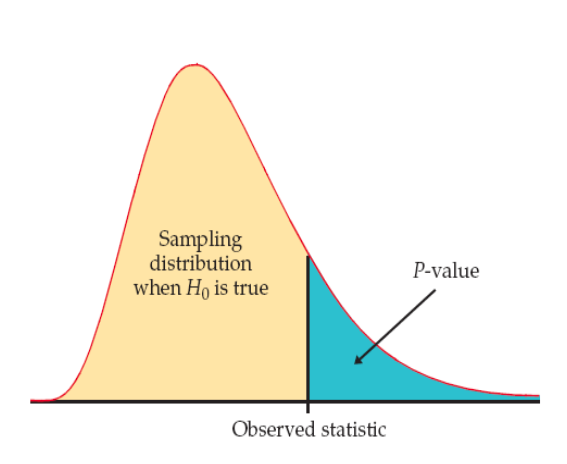
\includegraphics[width=8cm, height=4cm]{p-monte.png}
    		\end{center}
    	\end{figure}
\end{frame}

\begin{frame}
  \frametitle{Monte Carlo}
  \begin{theorem}[Moran's' I Monte Carlo Test]
The procedure is the following:

\begin{enumerate}
\item Rearrange the spatial data by shuffling their location and compute the Moran's I $S$ times. This will create the distribution under $H_0$.
\item Let $I_1^*, I_2^*,..., I_S^*$ be the Moran's I for each time. A consistent Monte Carlo p-value is then:
  \begin{equation}
    \widehat{p} = \frac{1 + \sum_{s=1}^S 1(I^*_s \geq I_{obs})}{S + 1}
  \end{equation}
  \item For tests at the $\alpha$ level or at $100(1- \alpha)\%$ confidence intervals, there are reasons for choosing $S$ so that $\alpha(S + 1)$ is an integer. For example, use $S=999$ for confidence intervals and hypothesis tests when $\alpha = 0.05$.
\end{enumerate}
\end{theorem}
\end{frame}

\begin{frame}
  \frametitle{Inference}
  Inference:
    \begin{itemize}
      \item If $I > \E(I)$, then a spatial unit tends to be connected by locations with similar attributes: Spatial clustering (low/low or high/high). The strength of positive spatial autocorrelation tends to increase with $I-\E(I)$.
      \item If $I < \E(I)$ observations will tend to have dissimilar values from their neighbors: Negative spatial autocorrelation (low/high or high/low)
    \end{itemize}
\end{frame}

\begin{frame}
  \frametitle{Application}
    \begin{itemize}
      \item \code{Lab1A.R}
      \item \code{Lab1B.R}
    \end{itemize}
\end{frame}

\end{document}


